\documentclass[11pt,a4paper]{article}
\usepackage[T1]{fontenc}
\usepackage{lmodern}
\usepackage[margin=25mm]{geometry}
\usepackage{microtype}
\usepackage{amsmath,amssymb,mathtools}
\usepackage{booktabs,array}
\usepackage{xcolor}
\usepackage{tikz,pgfplots}
\pgfplotsset{compat=1.18}
\usepackage{hyperref}
\definecolor{ink}{HTML}{203D57}
\definecolor{curveblue}{HTML}{206B99}
\definecolor{curvered}{HTML}{AF4B3D}
\hypersetup{colorlinks=true,linkcolor=ink,urlcolor=ink,pdftitle={When Quantum Training Loss Certifies a Quantum Operation},pdfauthor={},pdfsubject={Anonymous explanatory report},pdfcreator={LaTeX},pdfproducer={},pdfkeywords={}}
\pdfinfoomitdate=1
\pdftrailerid{}
\newcommand{\ket}[1]{\lvert #1\rangle}
\newcommand{\bra}[1]{\langle #1\rvert}
\newcommand{\Tr}{\operatorname{Tr}}
\newcommand{\normF}[1]{\left\lVert #1\right\rVert_{\mathrm F}}
\newcommand{\id}{\operatorname{id}}
\newcommand{\abs}[1]{\left\lvert #1\right\rvert}
\newcommand{\norm}[1]{\left\lVert #1\right\rVert}
\setlength{\parindent}{0pt}
\setlength{\parskip}{4.5pt plus 1pt}
\setlength{\emergencystretch}{2em}
\setlength{\abovedisplayskip}{9pt plus 2pt minus 2pt}
\setlength{\belowdisplayskip}{9pt plus 2pt minus 2pt}
\allowdisplaybreaks[1]
\widowpenalty=10000
\clubpenalty=10000
\raggedbottom
\numberwithin{equation}{section}
\begin{document}
\begin{center}
{\LARGE\bfseries\color{ink} When Quantum Training Loss\\[3pt] Certifies a Quantum Operation}\par
\vspace{5pt}
{\large An explanatory report}
\end{center}
\vspace{3pt}
\begin{abstract}
A suitable finite collection of test inputs can force a perfectly agreeing quantum channel to equal a unitary target. A small nonzero loss on those same inputs may nevertheless give a weak accuracy guarantee. The missing distinction is sensitivity to dissipative errors. This report develops a geometric criterion for when pure-state training loss controls average error linearly, derives its optimal coefficient, and explains the precision cost of menus that fail the criterion. The same geometry determines an optimal certification law even when the verifier chooses later probes adaptively and stores outputs in quantum memory. An independent-channel example makes the consequence explicit: adding a third global product input changes the required number of examples from order $n/\delta^2$ to order $1/\delta$, at fixed confidence, for an array of $n$ qubits and a requested average-error threshold $\delta$. Exact physical assumptions and the cost of each example remain part of the statement.
\end{abstract}

\paragraph{How to read the report.}
The starting point is basic vectors, matrix multiplication, and probability.
The quantum notation is introduced through one-qubit examples below.
For a first reading, follow the experiment, the numerical preview, the
statements of the bounds, and the certification recipes. The longer
calculations are marked as technical proofs; their purpose is explained
before their algebra begins. They establish the exact constants and remain
available for a second reading.

\section{The experiment and the two errors}
\label{sec:experiment}

Suppose an implemented operation is trained or calibrated on a finite collection of quantum states. Each chosen input has an ideal output, and a test asks whether the device produces that output. A natural hope is that a small average failure rate on these inputs means that the operation is accurate on an input it has never seen. The hope raises two separate questions. What does the true training loss imply about the operation? How many new device calls are needed to certify that implication? The first is a deterministic inequality between two errors. The second is an experiment with a confidence requirement.

The distinction is already visible for one qubit, a two-dimensional quantum system. Two nonorthogonal pure states can identify a target unitary exactly among all physical channels. Nevertheless, a weak dissipative error can be almost invisible to their survival tests. The error on general inputs is then proportional to a small noise strength, whereas the observed failure probability is proportional to its square. An additional input can expose the missing first-order signal. The central task is to determine precisely which input geometries have this property.

\subsection{States, channels, and the target}

For one qubit, begin with two column vectors and their equal superposition:
\[
 \ket0=\begin{pmatrix}1\\0\end{pmatrix},\qquad
 \ket1=\begin{pmatrix}0\\1\end{pmatrix},\qquad
 \ket+=\frac{\ket0+\ket1}{\sqrt2}
       =\frac1{\sqrt2}\begin{pmatrix}1\\1\end{pmatrix}.
\]
A ket $\ket\psi$ is a column vector; its matching bra $\bra\psi$ is the
conjugate-transposed row. Normalization means $\bra\psi\psi\rangle=1$:
the squared magnitudes of the entries sum to one. In dimension $d\ge2$,
the same notation describes vectors with $d$ complex entries. Their vector
space $\mathbb C^d$ is called the system's Hilbert space.

The identity matrix $I$ leaves every vector unchanged. The adjoint
$A^\dagger$ is the conjugate transpose of $A$, and $\Tr A$ is the sum of
its diagonal entries. The projector $P=\ket\psi\bra\psi$ keeps the component
along $\ket\psi$ and removes perpendicular components. Multiplying
$\ket\psi$ by an overall phase does not change $P$ or its physical state;
this phase-independent direction is called a ray.

A general, possibly mixed state is represented by a density matrix $\rho$.
It is positive and has trace one: $\rho=\rho^\dagger$ and its eigenvalues
are nonnegative. For example,
$\rho=\tfrac12\ket0\bra0+\tfrac12\ket1\bra1=I/2$ describes an equally
weighted mixture of the two basis states. A pure state has density matrix
$P=\ket\psi\bra\psi$. The trace-one condition normalizes total probability.

A physical operation is modeled by a completely positive, trace-preserving map, abbreviated CPTP. It acts linearly on matrices and has a Kraus representation
\begin{equation}
 \mathcal V(X)=\sum_a V_aXV_a^\dagger,
 \qquad \sum_a V_a^\dagger V_a=I.
 \label{eq:intro-kraus}
\end{equation}
The final identity preserves total probability. Complete positivity ensures that the operation remains physical when the system is part of a larger quantum state. The Kraus matrices describe possible exchanges with an unobserved environment; the experiment does not receive their labels.

A channel therefore maps an input density matrix to an output density
matrix. Its Kraus representation is one way to calculate that output, not
a list of outcomes revealed to the verifier. The target is the operation
we want; the hypothesis or device channel is the operation being checked.

The target is a unitary $U$, satisfying $U^\dagger U=UU^\dagger=I$.

A unitary preserves vector lengths and inner products and can be reversed.
A general channel can leave a pure input mixed when an environment is ignored. The implemented channel may include dissipation, even though its target is unitary. It is convenient to write the relative channel
\begin{equation}
 \mathcal E(X)=U^\dagger\mathcal V(X)U.
 \label{eq:intro-relative}
\end{equation}
The ideal relative operation is the identity map $\id$. Equation~\eqref{eq:intro-relative} is a choice of coordinates for the analysis. The experimental comparison remains with $UPU^\dagger$, and does not require a supplied implementation of $U^\dagger$.

\subsection{Training survival and average test risk}

A fixed weighted ensemble consists of $N$ distinct normalized rays:
\begin{equation}
 S=\{(p_i,P_i):1\le i\le N\},
 \qquad p_i>0,\qquad \sum_i p_i=1.
 \label{eq:intro-ensemble}
\end{equation}
A probe is one chosen input state, and a menu or catalogue is the list
of allowed probes. One trial prepares a selected input, uses the device once,
and performs a yes/no comparison with the ideal output. For an output
state $\rho$, comparison with $P=\ket\psi\bra\psi$ passes with probability
\[
 \Pr(\mathrm{pass})=\Tr(P\rho)=\bra\psi\rho\ket\psi.
\]
For a pure output $\ket\phi$, this is $|\langle\psi|\phi\rangle|^2$.

For example, comparison with $\ket+\bra+$ passes certainly on $\ket+$,
but only half the time on $I/2$. An equal superposition and an equal mixture
are different states.
Record a failure as one and a pass as zero. Repeating the trial estimates
its failure probability. Thus a survival infidelity is simply the
probability of failing this particular comparison.

The probability $p_i$ specifies how often input $P_i$ is selected. The survival test for that input has failure probability
\begin{equation}
 e_i(\mathcal E)=1-\Tr[P_i\mathcal E(P_i)],
 \qquad \epsilon_S(\mathcal E)=\sum_i p_i e_i(\mathcal E).
 \label{eq:intro-training}
\end{equation}
The quantity $\epsilon_S$ is the true mean training loss. An empirical frequency estimates it; selecting a hypothesis using the same outcomes introduces a separate statistical dependence. Certification below uses fresh outcomes after the hypothesis has been fixed.

The intended test risk is the infidelity averaged uniformly over all pure inputs:
\begin{equation}
 R(\mathcal E)=\int \left[1-\bra\psi\mathcal E(\ket\psi\bra\psi)\ket\psi\right]d\psi.
 \label{eq:intro-haar}
\end{equation}
The normalized Haar measure $d\psi$ is the probability distribution unchanged by every unitary rotation. On a composite system it includes entangled inputs. It defines the accuracy criterion, without requiring those inputs in the certification experiment. Both losses are dimensionless. A small average risk describes this test distribution; it is different from a guarantee on the worst individual input.

\paragraph{A numerical preview of the hidden error.}
Take the target to be the identity and use only $\ket0$ and $\ket+$,
with equal sampling probabilities. The physical noise family constructed
in Section~\ref{sec:qubit-example}, at the dimensionless strength $t=0.02$,
has average test risk about $1.01\%$. Its two-input training loss is only
about $0.0000510$, or $51$ failures per million trials. Adding $\ket1$
and sampling the three inputs equally raises that same device's training
loss to about $0.00670$, or $6{,}700$ failures per million trials. The device
has not improved; the test has become more sensitive to its error.

The distinction is between a quantity proportional to $t$ near zero
(first order) and one proportional to $t^2$ (second order). Halving $t$
roughly halves the first quantity and quarters the second. The proof below
explains when this weak signal can occur and when another input removes it.
These numerical values describe the explicit family, while the resulting
loss inequalities apply to every channel in the stated model.

For later calculations, define the Frobenius norm $\normF A=\sqrt{\Tr(A^\dagger A)}$.

Equivalently, $\normF A^2=\sum_{j,k}|A_{jk}|^2$: it is the ordinary
Euclidean size of the list of matrix entries. If $K_a$ are Kraus matrices for $\mathcal E$, the Haar second-moment identity is
\begin{equation}
 \int\abs{\bra\psi A\ket\psi}^2d\psi
 =\frac{\normF A^2+\abs{\Tr A}^2}{d(d+1)}.
 \label{eq:intro-haar-moment}
\end{equation}
The tensor product $A\otimes B$ acts on the joint space of two systems. One way to understand the normalization is to average two copies of the pure-state projector. Rotational invariance gives
$\int P\otimes P\,d\psi=(I+\mathbb F)/[d(d+1)]$, where $\mathbb F$ swaps the two copies. The averaged two-copy projector has trace one. Contracting this identity with $A$ and $A^\dagger$ gives Eq.~\eqref{eq:intro-haar-moment}. Thus an average over infinitely many inputs reduces to traces of finite matrices.

The quantity
\begin{equation}
 F_e(\mathcal E)=\frac1{d^2}\sum_a\abs{\Tr K_a}^2,
 \qquad R(\mathcal E)=\frac d{d+1}[1-F_e(\mathcal E)]
 \label{eq:intro-entanglement-fidelity}
\end{equation}
is called entanglement fidelity relative to the identity. It is a useful algebraic expression for the risk, not an additional experimental input. In particular $0\le R\le d/(d+1)$. The next step expresses the training loss and this risk on the same space of matrices. That common representation will reveal both the missing error directions and the cost of resolving them.

\section{The geometry behind a useful training loss}
\label{sec:geometry}

Use the fixed ensemble, relative channel, and losses of Section~\ref{sec:experiment}. The dimension, rays, and positive weights remain fixed throughout the small-error limits in this section.

\subsection{Measuring the directions that the probes can see}

Consider a complex matrix $A$. Acting on a probe vector, it produces a part along that vector and a part perpendicular to it. Only the perpendicular part moves the vector out of its original ray. Define
\begin{align}
Q_S(A)
&=\sum_i p_i\|(I-P_i)A\ket{\psi_i}\|_2^2 \\
&=\sum_i p_i\left(\|A\ket{\psi_i}\|_2^2
       -|\bra{\psi_i}A\ket{\psi_i}|^2\right).
\end{align}
Here $\|v\|_2=\sqrt{v^\dagger v}$ is the ordinary vector norm. The nonnegative quadratic form $Q_S$ measures the visibility of a matrix direction to the probes. Adding a scalar matrix changes only the parallel part, so
\[
Q_S(A+zI)=Q_S(A),\qquad z\in\mathbb C.
\]

A physical channel has a representation
\[
\mathcal E(X)=\sum_a K_aXK_a^\dagger,
\qquad \sum_aK_a^\dagger K_a=I.
\]
The second identity expresses conservation of total probability. It gives $\sum_a\|K_a\ket{\psi_i}\|_2^2=1$ and therefore the exact identity
\[
\boxed{\epsilon_S(\mathcal E)=\sum_aQ_S(K_a).}
\]
The matrices $K_a$ need not individually be unitary. Allowing general matrices here is precisely what permits dissipative errors.

For intuition, $Q_S(A)$ adds the squared perpendicular motion separately on each probe. It does not average the motions first, so different probes cannot cancel one another's contributions. Zero value means that every perpendicular component vanishes. This positivity is what turns an experimental loss question into a common-eigenvector question. 

There is a similarly simple expression for the test risk. Remove the scalar part of each Kraus matrix:
\[
K_a^0=K_a-\frac{\Tr K_a}{d}I.
\]
Applying Eq.~\eqref{eq:intro-haar-moment} and using $\sum_a\normF{K_a}^2=d$ gives
\[
\boxed{R(\mathcal E)=\frac{1}{d+1}\sum_a\normF{K_a^0}^2.}
\]
Thus training and test errors evaluate the same channel matrices in two different ways. Training uses the probe-dependent form $Q_S$; testing measures the total size of their nonscalar parts. Both expressions are independent of the particular channel representation.

\subsection{A necessary and sufficient condition for linear control}

The matrices invisible to the probes form the space
\[
\mathcal A_S=\{A:A\ket{\psi_i}\in\mathbb C\ket{\psi_i}
                    \text{ for every }i\}.
\]
A nonzero vector $v$ is a right eigenvector of $A$ with eigenvalue $\lambda$ when $Av=\lambda v$. Every probe is such an eigenvector of every matrix in this space, possibly with different eigenvalues. Positive weights ensure that $Q_S(A)=0$ exactly when $A\in\mathcal A_S$. A scalar matrix $zI$ multiplies every vector by the same number, so it
moves no vector out of its ray. These matrices are always invisible.
We want the smallest detectable response among error directions of the
same size. Multiplying $A$ by a number scales both its squared size and
$Q_S(A)$ by that number's squared magnitude. We therefore set the size
to one. The constraint $\Tr A=0$, called tracelessness, removes the scalar
part. The minimum remaining response is the gap
\[
\mu_S=\min_{\substack{\Tr A=0\\\normF{A}=1}}Q_S(A).
\]
The minimization includes all complex matrices. A Hermitian matrix obeys $A=A^\dagger$, while a normal matrix obeys $AA^\dagger=A^\dagger A$. Neither restriction is imposed here. Hermitian matrices have orthogonal eigenspaces for distinct eigenvalues. General complex matrices can have nonorthogonal eigenvectors with different eigenvalues. That extra possibility is central here: two overlapping probe states can constrain a physical channel perfectly at zero loss while sharing an invisible direction of a non-Hermitian matrix. Restricting the minimization to Hermitian directions would remove the physical mechanism we need to test. The normalized directions form a closed, bounded set in a finite-dimensional space, and $Q_S$ is continuous. Its minimum is attained. If no direction has zero response, the minimum is strictly positive, so
\[
\mu_S>0\quad\Longleftrightarrow\quad\mathcal A_S=\mathbb CI.
\]

A positive gap yields, for every physical channel,
\[
\epsilon_S(\mathcal E)
=\sum_aQ_S(K_a^0)
\geq\mu_S\sum_a\normF{K_a^0}^2
=(d+1)\mu_SR(\mathcal E).
\]
Consequently the risk obeys a global linear inequality. Its smallest possible coefficient is
\[
\boxed{R(\mathcal E)\leq C_S\epsilon_S(\mathcal E),\qquad
C_S=\frac{1}{(d+1)\mu_S}.}
\]
A positive gap means that every nonscalar error direction leaves a detectable signal. A smaller positive gap gives a larger coefficient $C_S$, so the same measured loss permits a larger average test error. The displayed sum applies this comparison to every Kraus matrix of the channel.

The word global means that the inequality holds at every loss, not just near zero. The coefficient is finite exactly when the invisible space contains only scalar matrices.

To establish necessity and the exact coefficient, the potentially dangerous matrix must be embedded in a physical channel. For any nonscalar $L$, put $B=L^\dagger L$ and choose
\[
K_1(t)=\sqrt t\,L,\qquad K_0(t)=\sqrt{I-tB},
\qquad 0\leq t\leq\|L\|_{\mathrm{op}}^{-2}.
\]
The operator norm $\|L\|_{\mathrm{op}}$ is its largest singular value, and the square root is the positive matrix square root. The stated interval makes that square root well defined. Since $K_0^\dagger K_0+K_1^\dagger K_1=I$, this construction is exactly physical throughout the interval.

\begin{samepage}
The parameter $t$ is a dimensionless noise strength. For fixed $L$ as $t\downarrow0$, the notation $O(t^k)$ denotes a remainder bounded in magnitude, or matrix norm, by a constant times $t^k$. Expanding the square root gives
\begin{align}
\epsilon_S(\mathcal E_t)
 &=tQ_S(L)+\frac{t^2}{4}Q_S(L^\dagger L)+O(t^3),\\
R(\mathcal E_t)
 &=\frac{t}{d+1}\normF{L-\frac{\Tr L}{d}I}^2+O(t^2).
\end{align}
\end{samepage}
The remainder constants may depend on the fixed matrix and ensemble. If $\mu_S>0$, choose a traceless, Frobenius-normalized minimizing $L$. Then $R(\mathcal E_t)/\epsilon_S(\mathcal E_t)$ tends to $C_S$, proving sharpness. If instead a nonscalar $L$ is invisible, training loss is at most quadratic in $t$, while test risk has a positive linear term. No finite linear coefficient can then work.

The square root in $K_0(t)$ is an essential part of the construction. Choosing a small matrix perturbation without enforcing conservation of probability could produce an invalid channel and a false obstruction. Here $K_1$ introduces the desired error direction while $K_0$ compensates its probability cost exactly. When $L$ preserves all probe rays, the linear survival-loss term vanishes while the risk retains a positive linear term. The conclusion therefore concerns realizable noise rather than a merely algebraic direction outside the physical model.

\subsection{Exact identification and the three possible regimes}

The probes span the system when every state vector is a linear combination of them. Connect two probes by an edge when their inner product is nonzero; this means their state directions are not perpendicular. A graph is connected when a path of such edges joins any two vertices. This overlap graph answers the perfect-data question: the probes identify the identity among all physical channels exactly when they span the system and the graph is connected.

The reason follows directly from the channel matrices. Zero loss requires $K_a\ket{\psi_i}=\lambda_{ai}\ket{\psi_i}$. Conservation of probability implies
\[
\sum_a|\lambda_{ai}|^2=1,\qquad
\langle\psi_i|\psi_j\rangle
=\langle\psi_i|\psi_j\rangle
  \sum_a\overline{\lambda_{ai}}\lambda_{aj}.
\]
Across an overlap edge the two unit coefficient vectors have inner product one and must coincide. Connectivity makes them the same for every probe; spanning then makes each $K_a$ scalar. Notice the role of the entire collection of channel matrices in this argument. Each matrix is allowed its own eigenvalue on a given probe, but trace preservation ties the collection of eigenvalues together. That collective constraint can rule out all nonidentity channels at exactly zero loss even when the invisible matrix space is larger than the scalars. Robustness asks whether nearby physical channels can exploit that larger space, which is why exact identification alone does not settle it.

Conversely, missing a subspace leaves an undetectable relative phase on that subspace. Disconnected components span mutually orthogonal subspaces, on which different phases are likewise undetectable.

For small nonzero errors, a previously established bound supplies the other ingredient: connected spanning probes satisfy
\[
R(\mathcal E)\leq B_S\sqrt{\epsilon_S(\mathcal E)}
\]
with a finite ensemble-dependent constant $B_S$. Its proof represents the channel by a unitary interaction with an auxiliary environment. Each joint system-environment output is split into its ideal system component and a residual of norm at most $\sqrt{s}$, where $s=\max_i e_i$. Preservation of inner products controls the environmental overlaps along every edge. Following paths connects all probes, and an invertible basis of probe vectors extends the estimates to the whole system. This yields a test-risk bound of order $\sqrt{s}$. Since $s\leq\epsilon_S/p_{\min}$, with $p_{\min}=\min_i p_i>0$, it gives the displayed weighted bound near zero. Enlarging the constant covers the remaining losses, using $R\leq1$.

Define the worst compatible risk
\[
W_S(\varepsilon)=\sup_{\epsilon_S(\mathcal E)\leq\varepsilon}R(\mathcal E),
\]
where the supremum ranges over physical channels. There are exactly three regimes. Nonspanning or disconnected probes allow $W_S(0)>0$. Connected spanning probes with a nonscalar invisible matrix satisfy $W_S(\varepsilon)=\Theta_S(\sqrt\varepsilon)$. A scalar invisible space instead gives
\[
W_S(\varepsilon)=C_S\varepsilon+O_S(\varepsilon^2)
\qquad(\varepsilon\downarrow0).
\]
Here $\Theta_S$ denotes upper and lower bounds by positive constants depending on the fixed ensemble.

For the middle regime, the physical witness supplies the matching lower bound. Its quadratic loss coefficient is positive. Otherwise $L^\dagger L$ would also preserve every probe ray. Being Hermitian, it would have equal eigenvalues across overlap edges, hence would equal $cI$. A nonscalar $L$ with this property would be proportional to a unitary preserving all probes, contradicting connected spanning. Thus $\epsilon_S\sim\beta_Lt^2$ and $R\sim a_Lt$ for positive constants. Eliminating $t$ proves the square-root lower bound. In the linear regime, the minimizing witness instead has $\epsilon_S=\mu_St+O(t^2)$; solving for $t$ proves the stated leading slope. Neither argument specifies the entire finite-error curve.

The orders describe a practical difference in uncertainty amplification. A linear guarantee turns a tenfold reduction in sufficiently small training loss into a tenfold reduction of its worst-case risk bound. In the square-root regime, the comparable improvement in the bound is only the square root of ten. The constants remain important and depend on the chosen geometry. These statements compare loss values for a fixed menu; the separate question of how many device uses are needed to resolve those losses will introduce an additional statistical resource.

\subsection{Two probes that hide a first-order error}

\label{sec:qubit-example}
This is the noise family used in the numerical preview. We now give its
matrices, so the difference between a small test signal and a small actual
error can be checked directly.

The simplest example uses a qubit and equal weights on
\[
\ket{0},\qquad \ket{+}=\frac{\ket{0}+\ket{1}}{\sqrt2}.
\]
These vectors are independent and overlap, so perfect data identify the target. Nevertheless,
\[
L=\begin{pmatrix}0&1\\0&1\end{pmatrix}
\]
has both as right eigenvectors. The exact physical family is
\[
K_0=\begin{pmatrix}1&0\\0&r\end{pmatrix},\qquad
K_1=\sqrt t\,L,\qquad
r=\sqrt{1-2t},\qquad 0\leq t\leq\tfrac12.
\]
Its individual survival errors are
\[
e_0=0,\qquad e_+=\frac{(1-r)^2}{4},\qquad e_1=t.
\]
For the original two probes,
\[
\epsilon_{S_2}=\frac{(1-r)^2}{8},\qquad
R=\frac{1-r}{3}+\frac t6
 =\sqrt{2\epsilon_{S_2}}-\frac23\epsilon_{S_2}.
\]
This is an exact relation on the full parameter interval. Since $1-r$ is of order $t$, training loss is quadratic while test risk is linear. The output on $\ket{+}$ can itself change at first order: it is the survival loss whose first derivative vanishes.

Adding $\ket{1}$ detects this witness at first order because $e_1=t$. More strongly, equal weights on all three rays give
\[
\mu_{S_3}=\frac{2-\sqrt2}{6},\qquad
R\leq(2+\sqrt2)\epsilon_{S_3}
\]
for every physical channel. The extra probe removes all nonscalar invisible directions, rather than merely exposing one chosen example.

This example also separates the content of a quantum state from its usefulness as a constraint. The original menu already contains the equal superposition $\ket{+}$. The added state $\ket{1}$ is a basis state, yet it is the input that repairs the robustness exponent. Its value comes from the new relation it forces between existing matrix eigenvectors. Calling a probe more complicated or more strongly superposed does not determine the robustness of the complete menu.


\begin{figure}[tbp]
\centering
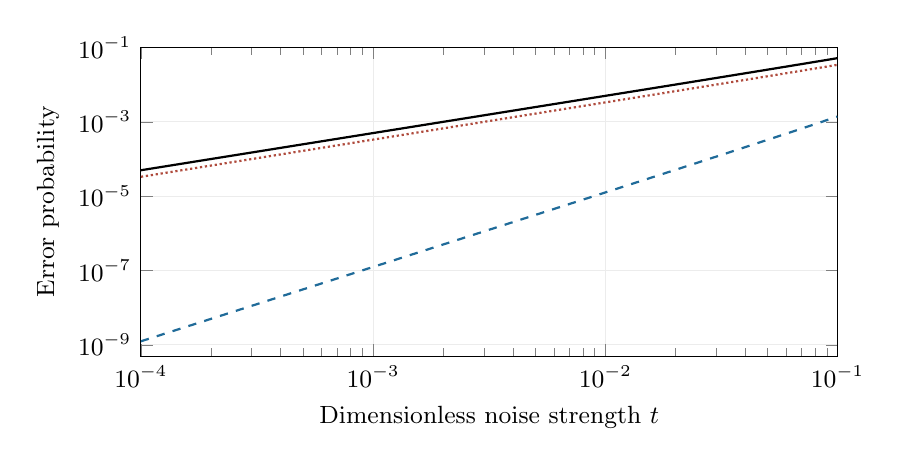
\begin{tikzpicture}
\begin{loglogaxis}[
 width=.86\textwidth,height=5.5cm,
 xmin=0.0001,xmax=0.1,ymin=0.0000000005,ymax=0.1,
 xlabel={Dimensionless noise strength $t$},ylabel={Error probability},
 grid=major,grid style={gray!15},
 tick label style={font=\small},label style={font=\small},
 samples=100,domain=0.0001:0.1]
\addplot[black,thick] {2*x/(3*(1+sqrt(1-2*x)))+x/6};
\addplot[curveblue,thick,dashed] {x*x/(2*(1+sqrt(1-2*x))^2)};
\addplot[curvered,thick,densely dotted] {(x*x/(1+sqrt(1-2*x))^2+x)/3};
\end{loglogaxis}
\end{tikzpicture}
\caption{The qubit family separates first- and second-order signals.
The average test risk $R$ (solid black) and the equal-weight three-input
loss $\epsilon_{S_3}$ (dotted red) are linear at small $t$; the equal-weight
two-input loss $\epsilon_{S_2}$ (dashed blue) is quadratic. Curves are
evaluated from the displayed Kraus operators. The gap theorem supplies
the corresponding channel-independent guarantees. Both axes are logarithmic: equal distances represent equal multiplication factors. As $t$ decreases, the quadratic signal falls faster than the linear signals.}
\label{fig:signal}
\end{figure}

\subsection{A direct test using basis coordinates}

First revisit the qubit. Choose $\ket0,\ket+$ as a basis. An operator can
preserve their rays while assigning them different eigenvalues. But
$\ket1=\sqrt2\ket+-\ket0$. Requiring this third vector to be an eigenvector
forces those first two eigenvalues to agree: its two nonzero basis
coefficients cannot acquire different multipliers. The operator must then
be a scalar matrix. The coordinate-support construction that follows records these forced equalities in larger menus.

The gap condition has a simple algebraic test. Extract any basis $b_1,\ldots,b_d$ from spanning probes, put $B=[b_1\ \cdots\ b_d]$, and express every additional probe as $\ket{\psi_i}=\sum_jc_{ij}b_j$. Construct a second graph, now on the $d$ basis indices: connect two indices whenever an additional probe has nonzero coordinates at both.

Every common right-eigenoperator must have the form $A=B\operatorname{diag}(\lambda_1,\ldots,\lambda_d)B^{-1}$. Writing $\zeta_i$ for the eigenvalue on additional probe $i$, its condition reads
\[
(\lambda_j-\zeta_i)c_{ij}=0.
\]
It forces equal diagonal eigenvalues wherever an extra probe connects basis coordinates. Consequently, if this coordinate-support graph has $m$ components, the invisible space has complex dimension $m$. In particular, it contains only scalars exactly when this graph is connected.

The distinction between the two graphs is essential. Overlaps enforce consistency between channel matrices at exactly zero loss. Coordinate support determines whether an individual matrix direction can escape a linear loss bound. A basis alone has $d$ isolated coordinate vertices, even if its overlap graph is connected. Adding one ray with all basis coordinates nonzero joins them all. More generally, several added rays suffice if their supports collectively connect every basis index.

The selected basis need not be orthogonal. A disconnected coordinate graph groups its basis vectors into complementary subspaces, each containing whole probe rays. These subspaces may meet at nonright angles. A matrix can multiply each subspace by a different number and remain invisible. This explains why a decomposition detected by coordinate support is more general than the orthogonal decomposition detected by disconnected overlaps. The two graphs encode distinct geometric constraints even when drawn from the same list of physical states.

\subsection{One extra uniform ray and the role of weights}

Consider the full orthonormal basis together with
\[
\ket{u}=\frac1{\sqrt d}\sum_{j=0}^{d-1}\ket{j}.
\]

A concrete minimal family in dimension $d$ consists of
$\ket1,\ldots,\ket{d-1}$ and the uniform vector $u$ just defined.
Its overlap graph is a connected star, so its $d$ rays identify exactly.
The nonscalar matrix $L=\sqrt d\ket u\bra0$ preserves all these rays,
and $L^\dagger L=d\ket0\bra0$ makes the physical witness valid for
$0\le t\le1/d$. This family exhibits the square-root regime in every fixed
dimension. Its allowed noise interval depends on dimension. The later
register theorem instead calibrates a product witness on a common interval
of global risk, uniformly in the number of qubits.

For the full $d+1$-ray menu, assign weight $b\in(0,1)$ to $\ket{u}$ and weight $a=(1-b)/d$ to each basis ray. The geometry guarantees a positive gap, but the gap's magnitude still matters. It sets how much experimental uncertainty can be amplified into test error.

For this fixed menu, uniform sampling gives a coefficient growing as $2d$
when $d$ grows. Optimizing the weights improves its leading growth to $d$.
For a qubit, weights $30\%,40\%,30\%$ on $\ket0,\ket+,\ket1$ give
coefficient $10/3$. The following calculation derives the exact formulas.

\subsubsection*{Technical calculation for the basis-plus-uniform menu}

To calculate it, let $\Pi_{\mathrm{off}}$ remove a matrix's diagonal entries and define the matrix-space projection
\[
\mathcal R_u(A)=(I-\ket{u}\bra{u})A\ket{u}\bra{u}.
\]
With the inner product $\langle A,B\rangle_F=\Tr(A^\dagger B)$, the operator representing $Q_S$ is $a\Pi_{\mathrm{off}}+b\mathcal R_u$. Choose an orthonormal basis $v_1,\ldots,v_{d-1}$ of $u^\perp$. For each basis vector $v$, split $\ket{v}\bra{u}$ into diagonal and off-diagonal parts. Their squared norms are $1/d$ and $(d-1)/d$. The resulting two-dimensional block is
\[
\begin{pmatrix}
b/d&b\sqrt{d-1}/d\\
b\sqrt{d-1}/d&a+b(d-1)/d
\end{pmatrix}.
\]
There are $d-1$ mutually orthogonal blocks. Their eigenvalues are
\[
\lambda_\pm=\frac{a+b\pm\sqrt{(a+b)^2-4ab/d}}{2}.
\]
The remaining nonscalar directions have eigenvalue $a$, with multiplicity $(d-1)^2$; the scalar direction has eigenvalue zero. Since $\lambda_-<a$, the gap is $\mu_S=\lambda_-$. Equal weights give
\[
\mu_S=\frac{1-\sqrt{1-1/d}}{d+1},\qquad
C_S=d+\sqrt{d(d-1)}.
\]

Weights can improve this coefficient. The gap is a minimum of functions linear in the weights, hence is concave. Averaging any assignment over permutations of the basis cannot decrease it. It therefore suffices to vary $b$, even when competitors may start with unequal basis weights. The smaller eigenvalue satisfies
\[
\mu^2-\frac{1+(d-1)b}{d}\mu+\frac{b(1-b)}{d^2}=0.
\]
It vanishes at both endpoints. Differentiation at an interior maximum gives $\mu=(1-2b)/[d(d-1)]$, and substitution yields
\[
b_* =\frac{1+\sqrt{d-1}}{d+1+2\sqrt{d-1}},\qquad
\mu_* =\frac{1}{d[d+1+2\sqrt{d-1}]}.
\]
Thus the optimized coefficient for this fixed menu is
\[
C_* =\frac{d[d+1+2\sqrt{d-1}]}{d+1}.
\]
For a qubit, weights $(3/10,4/10,3/10)$ on $(\ket{0},\ket{+},\ket{1})$ give $\mu_*=1/10$ and $C_*=10/3$. At large $d$, optimization improves the leading coefficient from approximately $2d$ to $d+2\sqrt d$. Adding a probe repairs the exponent; choosing weights improves its numerical cost. These are separate benefits, and this menu's coefficient still grows with dimension.


For an $n$-qubit register, $d=2^n$, every basis input and the uniform state $\ket{u}=\ket{+}^{\otimes n}$ can be prepared as a product of single-qubit states. Their simple preparation does not make the catalogue small: it still contains $2^n+1$ rays. The size of the catalogue, the cost of preparing one chosen ray, and the number of fresh outputs collected are distinct quantities. The gap calculation determines the loss-transfer coefficient for this catalogue, while its use in an experiment also requires that separate resource accounting.

\section{How many training rays support a strong guarantee?}
\label{dc:design}

The variance gap turns the design of a training experiment into a precise
geometric question.  A large gap means that every nontrivial operator direction
must disturb the available inputs appreciably.  We now ask how large that gap
can be when only a specified number of distinct pure inputs is available.
Allowing unequal sampling probabilities makes the question physically useful:
an experimenter can spend more calls on an informative input, but this freedom
does not remove the limitation imposed by the number of rays.

The bound optimizes the geometry and the sampling weights together. Its equality case explains why a symmetric arrangement is optimal even though no symmetry was assumed.

Write $\rho_S=\sum_i p_iP_i$ for the mean input state. The previously defined $Q_S$, $\mu_S$, and $C_S$ retain their meanings; set $C_S=+\infty$ when the gap vanishes.

\subsection{The support bound}

The sharp restriction is
\begin{equation}
 \mu_S=0\quad(N\leq d),\qquad
 \mu_S\leq\frac{N-d}{d(N-1)}
 \quad(d<N\leq d^2).
 \label{dc:support}
\end{equation}
Consequently,
\begin{equation}
 C_S\geq\frac{d(N-1)}{(d+1)(N-d)}
 \quad(d<N\leq d^2).
 \label{dc:support-coefficient}
\end{equation}
Equality in this range requires uniform weights and an equiangular tight
frame.  Here these words mean precisely
\begin{equation}
 \frac1N\sum_iP_i=\frac Id,
 \qquad
 \Tr(P_iP_j)=\frac{N-d}{d(N-1)}\quad(i\ne j).
 \label{dc:etf}
\end{equation}
The first condition distributes the mean input uniformly over the system
space.  The second makes every pair equally distinguishable by its squared
overlap.  Such frames attain the bound whenever they exist.  Their existence
depends on $d$ and $N$; the statement does not presume a frame for every pair
of parameters.

\paragraph{What this bound means.}
For $d=4$ and $N=5$, Eq.~\eqref{dc:support-coefficient} gives $C_S\ge16/5=3.2$.
No arrangement or weighting of those five rays has a smaller coefficient
valid for every channel. A different distinction appears for a qubit:
three optimally chosen rays attain $C_S=4/3$, while the fixed menu
$\ket0,\ket+,\ket1$ has best coefficient $10/3$. The number of inputs,
their geometry, and the choice of weights are separate design decisions.

\paragraph{The proof in three steps.}
First write the loss form as a matrix. Each ray then contributes one vector
to an auxiliary space. Second, use rank, the number of independent directions
in the columns of a matrix, to count those contributions. Third, remove any
advantage that might appear to come from an unbalanced mean input. The
resulting trace inequality limits the gap. The next calculation supplies
the exact bound; Section~\ref{dc:equality} identifies when equality is possible.

\subsubsection*{Technical proof of the support bound}
To prove the restriction without assuming a uniform mean input, regard
matrices as vectors. For a $2\times2$ matrix, column stacking turns its
entries into the four-component vector
$(A_{11},A_{21},A_{12},A_{22})^{\mathsf T}$. This is bookkeeping on matrices,
not preparation of an additional physical system. In dimension $d$, the
corresponding map is as follows.  Column vectorization is the map
\[
 a=\mathrm{vec}(A)=\sum_{j,k}A_{jk}\ket{k}\otimes\ket{j},
 \qquad a^\dagger\mathrm{vec}(B)=\Tr(A^\dagger B).
\]
Its first tensor factor represents the input index and its second the output
index.  Thus the space of all operators has dimension $d^2$ and its ordinary
vector inner product is the trace inner product of matrices.  Define
$w=\mathrm{vec}(I)$ and the following operators on this space:
\[
 \mathsf M=\sum_i p_i\mathrm{vec}(P_i)\mathrm{vec}(P_i)^\dagger,
 \qquad
 \Pi_{\rm sc}=\frac{ww^\dagger}{d},
 \qquad
 \mathsf Q=\rho_S^{\mathsf T}\otimes I-\mathsf M.
\]
The superscript $\mathsf T$ denotes transpose in the chosen basis, and
$\Pi_{\rm sc}$ projects onto the scalar-operator direction.  Let $I_{\rm op}$
denote the identity on the full operator space.  Direct substitution gives
\begin{equation}
 Q_S(A)=a^\dagger\mathsf Q a,
 \qquad
 \mathsf Q\succeq\mu_S(I_{\rm op}-\Pi_{\rm sc}),
 \qquad \mathsf Qw=0.
 \label{dc:operator-gap}
\end{equation}
Here $X\succeq Y$ means that $X-Y$ is positive semidefinite.  Also
$\Tr\mathsf M=1$, $\operatorname{rank}\mathsf M\leq N$, and
$\Tr\mathsf Q=d-1$.  Each training ray contributes only one rank-one term to
$\mathsf M$.  This rank restriction is the point at which catalogue size
enters the proof.

Vectorization is only a way to organize the quadratic form.  No physical
system of dimension $d^2$ is prepared.  A vector in this auxiliary space is
a matrix acting on the original system, and orthogonality to $w$ means that
the matrix is traceless.  The matrix $\mathsf Q$ records the squared motion
away from the selected rays in every such direction.  Its zero scalar
direction expresses the elementary fact that multiplying a state vector
by a scalar does not move it out of its ray.  The gap asks how much motion
is guaranteed after this irrelevant scalar direction has been removed.

First observe that $\mu_S\leq\lambda_{\min}(\rho_S)$.  Choose a normalized
minimum-eigenvalue vector $v$ of $\rho_S$ and a normalized $u$ perpendicular
to $v$.  The traceless operator $A=\ket{u}\bra{v}$ has Frobenius norm one,
and
\[
 Q_S(A)=\bra{v}\rho_S\ket{v}
 -\sum_i p_i|\langle\psi_i|u\rangle|^2
                 |\langle v|\psi_i\rangle|^2
 \leq\lambda_{\min}(\rho_S).
\]
In particular, inputs confined to a proper subspace have zero gap.

Assume now that $\mu_S>0$, and choose a temporary number
$0<\mu<\mu_S$.  The preceding observation makes
$B=\rho_S-\mu I$ strictly positive.  Put
\[
 D=B^{\mathsf T}\otimes I,
 \qquad H=D+\mu\Pi_{\rm sc}.
\]
Equation~\eqref{dc:operator-gap} gives $0\preceq\mathsf M\preceq H$.
The positive matrix $H^{-1/2}\mathsf M H^{-1/2}$ therefore has eigenvalues
at most one and rank at most $N$.  Its trace obeys
\begin{equation}
 N\geq\Tr(H^{-1}\mathsf M).
 \label{dc:rank-trace}
\end{equation}
We will lower-bound this trace using only $\Tr\rho_S=1$.

The rescaling by $H^{-1/2}$ is useful because the weighted input average may
favor some system directions over others.  Simply counting eigenvalues of
$\mathsf M$ would not remove that imbalance.  After this rescaling, however,
every nonzero eigenvalue is bounded by one.  The number of available rays
therefore limits their total trace.  A lower bound on that trace becomes a
lower bound on the number of rays required for any proposed positive gap.

Introduce the positive scalar quantities
\[
 s=\Tr B^{-1},\quad s_2=\Tr B^{-2},\qquad
 a=\Tr(\rho_SB^{-1})=d+\mu s,\qquad
 b=\Tr(\rho_SB^{-2})=s+\mu s_2.
\]
The inverse of $H$, obtained by adding its single rank-one term to $D$, is
\[
 H^{-1}=D^{-1}-\frac{\mu}{a}D^{-1}ww^\dagger D^{-1}.
\]
Taking its trace against $\mathsf M$ yields
\[
 \Tr(H^{-1}\mathsf M)
 =a-\frac{\mu}{a}
       \sum_i p_i\bra{\psi_i}B^{-1}\ket{\psi_i}^{\!2}.
\]
For a Hermitian matrix, its mean square on a normalized vector is at least
the square of its mean.  Applied to $B^{-1}$ and averaged over the probes,
this gives
\[
 \sum_i p_i\bra{\psi_i}B^{-1}\ket{\psi_i}^{\!2}
 \leq\sum_i p_i\bra{\psi_i}B^{-2}\ket{\psi_i}=b.
\]
Consequently $N\geq g_\mu$, where $g_\mu=a-\mu b/a$.

For the remaining scalar step, let $x_j=\lambda_j(\rho_S)-\mu>0$ and
$\tau=\sum_jx_j=1-d\mu$.  Thus $s=\sum_jx_j^{-1}$ and
$s_2=\sum_jx_j^{-2}$.  Two inequalities suffice:
\begin{equation}
 \tau s\geq d^2,\qquad
 \tau(s^2-s_2)\geq d(d-1)s.
 \label{dc:scalar-inequalities}
\end{equation}
The first follows by applying the inner-product inequality to
$(\sqrt{x_j})_j$ and $(1/\sqrt{x_j})_j$.  To see the second explicitly,
expand its left side into pair and triple contributions:
\begin{align*}
 \tau(s^2-s_2)
 &=2(d-1)s+
   2\sum_{i<j<k}\frac{x_i^2+x_j^2+x_k^2}{x_ix_jx_k}\\
 &\geq2(d-1)s+
   2\sum_{i<j<k}\left(\frac1{x_i}+\frac1{x_j}+\frac1{x_k}\right)
 =d(d-1)s.
\end{align*}
For every triple, the inequality is equivalent to the nonnegativity of
$(x_i-x_j)^2+(x_j-x_k)^2+(x_k-x_i)^2$.  When $d=2$, the triple sums are
empty and the second inequality is an equality.

Substituting $a=d+\mu s$ and $b=s+\mu s_2$ now gives
\begin{align*}
 a\tau\left[g_\mu-\frac{d(1-\mu)}{1-d\mu}\right]
 &=(d-1)\mu[-d^2+(1-2d\mu)s]
     +\tau\mu^2(s^2-s_2)\\
 &\geq(d-1)\mu(\tau s-d^2)\geq0.
\end{align*}
The first inequality uses the second part of
\eqref{dc:scalar-inequalities}; the last uses its first part.  Hence
\begin{equation}
 N\geq\frac{d(1-\mu)}{1-d\mu}.
 \label{dc:prelimit-support}
\end{equation}
Its right side exceeds $d$ whenever $\mu>0$, excluding a positive gap for
$N\leq d$.  For $N>d$, rearrange to
$\mu\leq(N-d)/[d(N-1)]$ and let $\mu$ increase to $\mu_S$.
This proves the support bound for arbitrary positive weights.

The calculation leaves little freedom hidden in the weight choice.  The
dependence on individual inputs disappeared through the nonnegative variance
of $B^{-1}$; the remaining dependence on the eigenvalues of their mean input
disappeared through \eqref{dc:scalar-inequalities}.  These are inequalities
valid for every positive spectrum with the prescribed trace.  Thus an
unbalanced mean state cannot create an exceptional design outside the bound.
The equality conditions will recover precisely where these two possible
sources of slack can both disappear.

\subsection{Why equality enforces a symmetric experiment}

\label{dc:equality}
The conclusion of this subsection is simple: attaining the support bound
forces uniform sampling, a uniform mean input, and equal pairwise overlaps.
The calculation checks both the possible singular endpoint and the equality
conditions. These details ensure that a nonsymmetric or unbalanced ensemble
cannot evade the conclusion.

Suppose $d<N\leq d^2$ and the bound is attained, and write
$q=(N-d)/[d(N-1)]=\mu_S$.  Equality cannot simply be substituted into
an inverse that might become singular.  The proof above retains the useful
quantitative slack
\[
 g_\mu-\frac{d(1-\mu)}{1-d\mu}
 \geq\frac{(d-1)\mu(\tau s-d^2)}{(d+\mu s)\tau}.
\]
If $\lambda_{\min}(\rho_S)=q$, then $s$ diverges as $\mu$ increases to
$q$.  Since $1-dq>0$, the right side tends to $d-1$.  The subtracted
quantity tends to $d(1-q)/(1-dq)=N$, contradicting $N\geq g_\mu$.
Thus $\lambda_{\min}(\rho_S)>q$, and all inverse matrices remain defined
at the endpoint.

At $\mu=q$, every inequality leading to
\eqref{dc:prelimit-support} must be an equality.  The slack therefore forces
$\tau s=d^2$.  Equality in the first scalar inequality requires all $x_j$
to coincide, so $\rho_S=I/d$.  A balanced mean input is therefore a
consequence of optimality, rather than an assumption made in proving it.

Now $\mathsf M w=w/d$ and $\mathsf Q=I_{\rm op}/d-\mathsf M$.
On the traceless subspace, every eigenvalue of $\mathsf M$ is at most
\[
 \kappa=\frac1d-q=\frac{d-1}{d(N-1)}.
\]
That part of $\mathsf M$ has rank at most $N-1$ and trace $(d-1)/d$.
Its trace is exactly $(N-1)\kappa$, forcing $N-1$ nonzero eigenvalues,
each equal to $\kappa$.

The $N\times N$ Gram matrix
$G_{ij}=\sqrt{p_ip_j}\Tr(P_iP_j)$ has the same nonzero eigenvalues as
$\mathsf M$.  With $v=(\sqrt{p_1},\ldots,\sqrt{p_N})^{\mathsf T}$,
balance gives $Gv=v/d$.  The remaining $N-1$ eigenvalues are
$\kappa$, so
\[
 G=\kappa I_N+(1/d-\kappa)vv^\dagger.
\]
Its diagonal entries give
$p_i=\kappa+(1/d-\kappa)p_i$, hence $p_i=1/N$.  Its off-diagonal
entries give $\Tr(P_iP_j)=1/d-\kappa=q$.  These are precisely
\eqref{dc:etf}.  Conversely, those frame conditions yield this Gram matrix
and the stated spectrum, so the gap is $q$.  Both necessity and sufficiency
follow, including $N=d^2$.

The conclusion concerns symmetry of projectors rather than phases of state
vectors.  Replacing any $\ket{\psi_i}$ by a phase multiple changes neither
the preparation nor any equation above.  Equal pairwise squared overlaps
and a uniform mean state are the physically relevant properties.  They
ensure that the available probes distribute sensitivity evenly among the
operator directions that their number can cover.  A merely balanced
ensemble can still have a smaller gap if its pairwise geometry leaves
one direction weakly tested.

\subsection{The absolute optimum}

No pure-state catalogue can have a global coefficient smaller than one.
Equality holds precisely when its weighted inputs reproduce the two-copy
average of uniformly distributed pure states. At least $d^2$ rays are needed.
Such an ensemble is called a weighted projective $2$-design. The next proof
expresses that second-moment condition using the matrix notation from the
support proof.

\subsubsection*{Technical proof of the absolute optimum}

Regardless of $N$, the positive matrix $\mathsf Q$ has trace $d-1$,
one zero scalar direction, and $d^2-1$ traceless directions.  Their smallest
eigenvalue cannot exceed their average:
\[
 \mu_S\leq\frac{d-1}{d^2-1}=\frac1{d+1}.
\]
Equality requires
$\mathsf Q=(I_{\rm op}-\Pi_{\rm sc})/(d+1)$.  The partial trace discards one tensor factor by summing its diagonal matrix elements. Taking it
over the output factor of this identity, using
$\Tr_{\rm out}\mathsf Q=(d-1)\rho_S^{\mathsf T}$, forces
$\rho_S=I/d$.  Substitution then gives
\[
 \mathsf M=\frac{I_{\rm op}+ww^\dagger}{d(d+1)}.
\]
Transposing only the input factor converts this identity into
\begin{equation}
 \sum_i p_iP_i\otimes P_i=\frac{I_{\rm op}+\mathbb F}{d(d+1)},
 \label{dc:design-moment}
\end{equation}
where $\mathbb F$ exchanges the two factors.  Equation~\eqref{dc:design-moment}
defines a weighted complex projective $2$-design: its second moment equals
the second moment of uniformly distributed pure states.  Conversely, that
moment identity gives the optimal gap.  The corresponding $\mathsf M$ has
full rank $d^2$, so at least $d^2$ distinct rays are necessary.

Matching a second moment is enough here because the survival loss is
quadratic in the state projector.  Equation~\eqref{dc:design-moment} allows
that quadratic average to be computed exactly from a finite weighted set.
The experiment need not actually draw a continuous random pure state.
The input catalogue replaces that average for the quantities used in the
loss relation.  Its weights are part of the construction and need not be
uniform when the catalogue is larger than the minimal cardinality.

\paragraph{Interpretation and an attaining construction.}

The best possible coefficient is therefore $C_S=1$.  A smaller catalogue
can still be useful, but its coefficient carries an unavoidable penalty.
For $N=d+k\leq d^2$, the bound reads
\[
 C_S\geq\frac{d(d+k-1)}{(d+1)k}.
\]
When $k$ is small compared with $d$, the penalty is of order $d/k$.
One extra ray can make a finite linear guarantee possible while leaving its
coefficient large.  This distinguishes repairing the precision exponent from
making the experiment well conditioned.


The minimal linear-robust support $N=d+1$ has an explicit attaining example:
\[
 \ket{\phi_k}=\frac1{\sqrt d}\sum_{j=0}^{d-1}
       e^{2\pi\mathrm i jk/(d+1)}\ket j,
 \qquad k=0,\ldots,d,
 \qquad p_k=\frac1{d+1}.
\]
Here $\mathrm i^2=-1$. Summing the phases gives a mean projector $I/d$
and squared overlaps $1/d^2$ for distinct rays. The support theorem therefore
gives $\mu_S=1/d^2$ and $C_S=d^2/(d+1)$. This example also separates a
small number of simple preparation choices from a coefficient independent
of dimension: the minimal-support optimum still grows with $d$.


\section{How a physical noise promise changes robustness}

The distinction between a unitary target and a general channel hypothesis is physically consequential. A unitary error moves amplitudes coherently. A dissipative error can also move probability into an inaccessible environment. A training menu that detects every coherent direction can still be insensitive, to first order in the noise strength, to an allowed dissipative direction. We now quantify which part of this obstruction disappears when the channel is known to be unital, and how it returns when a small deviation from unitality is permitted.

\subsection{The commutator gap and a sharp unital bound}

For a qubit, $I/2$ is an input with no preferred basis direction. Unitality
means that this state remains $I/2$ after the channel. Individual pure inputs
can still change substantially. The useful additional constraint is on
how probability can flow in both directions between a probe ray and its
perpendicular space.

A channel is unital when $\mathcal E(I)=I$, or equivalently when it preserves the maximally mixed state $I/d$. This includes unitary channels and many noisy channels. Composing with the inverse target unitary in the mathematical description preserves this property. Assume throughout this subsection that the probe rays span $\mathbb C^d$, their overlap graph is connected, and their weights are positive. The commutator is $[A,P]=AP-PA$. Write
\[
 \rho_S=\sum_i p_iP_i,
 \qquad
 G_S(A)=\frac12\sum_i p_i\normF{[A,P_i]}^2,
 \qquad
 \gamma_S=\min_{\substack{\Tr A=0\\\normF{A}=1}}G_S(A).
\]
The minimization still allows arbitrary complex matrices. Unlike the one-sided variance $Q_S$, the commutator form checks how the operator acts both from and into a probe ray. Expanding a rank-one projector gives
\begin{align*}
 \normF{[A,P_i]}^2
 &=\bra{\psi_i}A^\dagger A\ket{\psi_i}
  +\bra{\psi_i}AA^\dagger\ket{\psi_i}
  -2\left|\bra{\psi_i}A\ket{\psi_i}\right|^2,\\
 G_S(A)&=\tfrac12\bigl[Q_S(A)+Q_S(A^\dagger)\bigr].
\end{align*}

For one term, take $P=\ket0\bra0$ and $A=\ket0\bra1$.
Then $A\ket0=0$, so its one-ray variance is zero, whereas
$A^\dagger\ket0=\ket1$ gives variance one. The symmetrized expression
sees this reverse motion even when the one-sided variance does not.

Unitality does not say that each input state is unchanged. It says that a completely mixed input acquires no preferred direction. A noisy mixture of unitary operations can satisfy this condition while substantially disturbing individual pure states. The commutator measures sensitivity to such disturbances by comparing an operator with the projector defining a test. Its symmetrization is essential: the one-sided variance can vanish because every probe is a right eigenvector, while the adjoint can still move those same vectors out of their rays. The two forms therefore encode different restrictions on the physically permitted error.

Here $\gamma_S>0$. To see why, a matrix commuting with every $P_i$ acts on each probe with an eigenvalue $\lambda_i$, on both the left and the right. A nonzero overlap implies
\[
 \lambda_i\langle\psi_i|\psi_j\rangle
 =\bra{\psi_i}A\ket{\psi_j}
 =\lambda_j\langle\psi_i|\psi_j\rangle.
\]
Connectivity makes all eigenvalues equal, and spanning then makes the matrix scalar. Thus the commutator form has no traceless kernel. Conversely, failure of spanning or connectivity leaves a nontrivial orthogonal projection commuting with all probes. The commutator gap therefore detects precisely the connected-spanning identification condition.

Trace preservation turns this operator observation into an exact channel identity:
\begin{equation}
 \sum_aG_S(K_a)
 =\epsilon_S(\mathcal E)
  +\frac12\Tr\!\left[\rho_S\bigl(\mathcal E(I)-I\bigr)\right].
 \label{eq:physical-commutator-identity}
\end{equation}
Indeed, the first quadratic term in the expansion sums to one on each normalized input because $\sum_aK_a^\dagger K_a=I$. The second sums to the expectation of $\mathcal E(I)$, fixing the sign of the correction. Subtracting scalar parts from the Kraus operators does not change their commutators. The Haar-risk identity consequently implies
\[
 (d+1)\gamma_SR(\mathcal E)
 \le\sum_aG_S(K_a).
\]
For a unital channel the correction in \eqref{eq:physical-commutator-identity} vanishes, and hence
\begin{equation}
 R(\mathcal E)\le\frac{\epsilon_S(\mathcal E)}{(d+1)\gamma_S}.
 \label{eq:physical-unital-bound}
\end{equation}
This remains linear even when the unrestricted variance gap $\mu_S$ is zero.

The coefficient is sharp within the unital class. If $A=X+iY$ with $X,Y$ traceless and Hermitian, then
\[
 \normF{A}^2=\normF{X}^2+\normF{Y}^2,
 \qquad G_S(A)=G_S(X)+G_S(Y).
\]
The commutators with a Hermitian projector are anti-Hermitian, so the relevant cross term vanishes. A normalized Hermitian minimizer $H$ therefore exists. The unitary $V_s=e^{isH}$ produces
\[
 \epsilon_S(V_s\,\cdot\,V_s^\dagger)=s^2\gamma_S+O(s^3),
 \qquad R(V_s\,\cdot\,V_s^\dagger)=\frac{s^2}{d+1}+O(s^3).
\]
Their ratio approaches the coefficient in \eqref{eq:physical-unital-bound}. Restricting a hypothesis to unitary noise can therefore be quantitatively correct for that restricted class while missing a dissipative obstruction in the implemented device.

This sharpness argument has a useful interpretation. The commutator bound applies globally to every unital channel, but its best coefficient is already determined arbitrarily close to the target by coherent perturbations. No elaborate dissipative example is needed to attain that limiting ratio. As with the unrestricted coefficient, sharpness of the linear inequality does not mean that a straight line describes the whole feasible boundary at finite error. It identifies the strongest coefficient that can hold without further information about the channel or its error magnitude.

\subsection{A nonunitality budget and the joint error frontier}

The trace norm $\|X\|_1=\Tr\sqrt{X^\dagger X}$ is the sum of the singular values. Measure deviation from unitality by
\[
 u(\mathcal E)=\frac12\left\|\mathcal E(I/d)-I/d\right\|_1.
\]
Let $\Delta=\mathcal E(I)-I$. Trace preservation gives $\Tr\Delta=0$ and $\|\Delta\|_1=2d\,u(\mathcal E)$. Subtracting the midpoint of the extreme eigenvalues of $\rho_S$ inside the trace yields
\[
 \Tr(\rho_S\Delta)
 \le d\bigl[\lambda_{\max}(\rho_S)
             -\lambda_{\min}(\rho_S)\bigr]u(\mathcal E).
\]
Together with the exact identity, this proves the global inequality
\begin{equation}
 R(\mathcal E)\le
 \frac{\epsilon_S(\mathcal E)
  +\frac d2\bigl[\lambda_{\max}(\rho_S)
             -\lambda_{\min}(\rho_S)\bigr]u(\mathcal E)}
 {(d+1)\gamma_S}.
 \label{eq:physical-nonunital-bound}
\end{equation}
For a balanced ensemble, $\rho_S=I/d$, the correction vanishes for every channel. In that case $Q_S(A)=Q_S(A^\dagger)=G_S(A)$, and $\mu_S=\gamma_S$. A connected-spanning ensemble with $\mu_S=0$ must consequently be unbalanced.

The practical question is now: if the training loss is at most
$\varepsilon$, and a maximally mixed input changes by at most $\eta$ in
trace distance, how large could the average error still be? Both tolerances
are physical promises about the same fixed channel.

To make the two error budgets explicit, define
\[
 \Phi_S(\varepsilon,\eta)
 =\sup\{R(\mathcal E):\epsilon_S(\mathcal E)\le\varepsilon,
                       \ u(\mathcal E)\le\eta,\ \mathcal E\text{ CPTP}\}.
\]
For a fixed connected-spanning ensemble in the singular regime $\mu_S=0$,
\begin{equation}
 \Phi_S(\varepsilon,\eta)
 =\Theta_S\!\left(\varepsilon+\min\{\eta,\sqrt\varepsilon\}\right).
 \label{eq:physical-frontier}
\end{equation}
The comparison holds for sufficiently small $\varepsilon$, uniformly over $\eta\ge0$; its constants depend on the ensemble and dimension. The upper bound combines \eqref{eq:physical-nonunital-bound}, which gives order $\varepsilon+\eta$, with the connected-spanning square-root bound, which gives order $\sqrt\varepsilon$.

Two physical families prove the matching lower bound. A depolarizing channel
\[
 \mathcal D_q(X)=(1-q)X+q\Tr(X)I/d
\]
with $0\le q\le1$ is unital and has $R=\epsilon_S=q(d-1)/d$. It realizes risk $\varepsilon$ while using none of the nonunitality budget. For the other contribution, choose a traceless, normalized nonscalar common right-eigenoperator $L$. The exact Kraus family
\[
 K_1=\sqrt t\,L,
 \qquad K_0=\sqrt{I-tL^\dagger L}
\]
satisfies $\epsilon_S\le B_Lt^2$ and $R\ge a_Lt$ at small $t$, for positive fixed constants. Its deviation from unitality is exactly
\[
 \mathcal E_t(I)-I=t(LL^\dagger-L^\dagger L),
 \qquad u(\mathcal E_t)=\nu_Lt,
 \qquad \nu_L=\frac{\|LL^\dagger-L^\dagger L\|_1}{2d}>0.
\]
Positivity follows because a normal operator with these connected, spanning eigenvectors would be scalar. Choosing $t$ to be a sufficiently small constant times $\min\{\sqrt\varepsilon,\eta\}$ respects both budgets and produces that order of risk. The larger of the two lower bounds is at least half their sum, proving \eqref{eq:physical-frontier}. If $\mu_S>0$, unrestricted linear robustness instead gives $\Phi_S=\Theta_S(\varepsilon)$ for all $\eta\ge0$.

Exact unitality, or a budget $\eta$ of order $\varepsilon$, preserves linear robustness. Every fixed positive budget eventually admits square-root behavior as $\varepsilon$ tends to zero. Such a budget is an independently justified physical promise. Estimating it can require preparations and measurements absent from the training menu.

The frontier separates three scales without requiring a numerical crossover fit. When the nonunitality budget is no larger than a constant times the training tolerance, both contributions are linear in that tolerance. At intermediate budgets between the training tolerance and its square root, the allowed nonunitality sets the larger contribution to the worst compatible risk. Once the budget reaches the square-root scale, making it larger no longer changes the asymptotic order because the identifying menu itself supplies the square-root upper bound. These comparisons keep the geometry and dimension fixed. They do not assert that their implicit constants remain controlled for a sequence of increasingly ill-conditioned menus.


\section{What the gap means for the number of experiments}
\label{dc:certification}

A deterministic loss inequality relates two properties of the same channel.
A certification experiment must infer whether a channel is acceptable from
random measurement outcomes.  To connect the two, consider a fixed target
unitary channel $\mathcal U$ and a fixed, memoryless device channel
$\mathcal V$.  In relative coordinates write
$\mathcal E=\mathcal U^\dagger\circ\mathcal V$.  The statistical task is
to distinguish
\[
 H_0:\mathcal E=\id
 \qquad\text{from}\qquad
 H_1:R(\mathcal E)\geq\delta,
\]
with probability at most $\alpha$ of rejecting the target and probability
at most $\alpha$ of accepting any permitted alternative.  Here
$\delta>0$ is the risk separation and $0<\alpha<1/2$ is the allowed error
probability.  The resource $T$ is a worst-case cap on device calls.

On the exact target, the probability of rejection must be at most $\alpha$. On every device with $R\ge\delta$, the probability of acceptance must be at most $\alpha$. An imperfect channel with
$0<R<\delta$ lies between these promised cases; either decision is allowed
there.
All logarithms below are natural logarithms.

Keep the probabilities distinct:
\begin{center}
\begin{tabular}{@{}p{.20\textwidth}p{.72\textwidth}@{}}
\toprule
Symbol & Meaning in the experiment \\
\midrule
$\epsilon_S$ & True mean failure probability on the chosen probes. \\
$\varepsilon$ & A permitted upper tolerance on that training loss. \\
$\delta$ & Risk threshold above which the device must be rejected. \\
$\alpha$ & Allowed probability of a wrong certification decision. \\
$T$ & Maximum number of fresh calls to the device. \\
\bottomrule
\end{tabular}
\end{center}
For example, $\delta=0.01$ and $\alpha=0.05$ ask for a test that mistakenly
accepts any device with risk at least $1\%$ with probability at most $5\%$.
This guarantee concerns repeated applications of the test, not a posterior
probability assigned to one accepted device.

Each call receives a fresh prescribed input $P_i$, chosen by a classical
label.  The verifier may use its previous outputs and arbitrary quantum
memory to choose that label, retain outputs coherently, and make a final
joint measurement.  Conditional on the chosen label, the new input is
independent of retained memory.  This independence defines the experiment:
it supplies no memory-entangled input, coherent superposition of menu labels,
or return of an earlier output through the device.  The device environment
remains inaccessible.  For the matching upper bound, the verifier can test
the ideal output projector $UP_iU^\dagger$.  State preparation and the
implementation of that measurement are separate physical costs.

The risk threshold concerns the full device, and the error guarantee must
hold for every fixed alternative above that threshold.  A successful test
therefore certifies a channel property rather than merely fitting an
observed sample.  If a learning procedure selected the device hypothesis
using previous data, these certification outcomes are collected afresh
after that choice.  Their independence is what permits a fixed-channel
statistical guarantee.  The total experiment may use fewer than its cap
when a failure appears early, but its advertised resource guarantee covers
the longest branch as well as typical branches.

An elementary version of the statistical mechanism is already visible.
If one test fails with probability $q$ under an alternative and never fails
under the target, accepting after $T$ consecutive passes makes the error
probability $(1-q)^T$.  For small $q$ this is approximately $e^{-Tq}$, so
the number of repetitions is approximately $\log(1/\alpha)/q$.  With the sampling weights optimized, denote the best gap by $\mu_*$, formally defined next. The loss
inequality supplies a guaranteed signal $q\geq(d+1)\mu_*\delta$.  What
remains to prove is that a more elaborate experiment cannot extract a
better leading signal from the same menu.  The next construction supplies
exactly that converse.

\paragraph{The attainable experiment.}
Assume the optimized gap is positive. Independently choose a probe using
the optimized weights, call the device, and test its ideal output ray.
Reject as soon as any trial fails. Accept only if all $T$ trials pass.
The ideal device always passes. A bad device has mean rejection probability
at least $c\delta$, where $c=(d+1)\mu_*$. Thus its probability of passing
all trials is at most $(1-c\delta)^T$. For small $\delta$, about
$\log(1/\alpha)/(c\delta)$ trials suffice. The finite bound below gives
the exact rounding and probability formula. The remaining task is to show
why a more elaborate allowed verifier cannot improve the leading cost.

\subsection{One alternative that is hard for every label}

\paragraph{What the converse must accomplish.}
An adaptive verifier can change its next input after seeing earlier outputs.
A lower bound must therefore supply one fixed bad channel that is hard to
detect on every input, not a new channel chosen after each label. The
minimax calculation below finds such a simultaneous weak disturbance.
Its physical realization then uses the exact Kraus construction already
introduced in Section~\ref{sec:geometry}.

\subsubsection*{Technical construction of the common alternative}

For a fixed menu, optimize the sampling probabilities:
\[
 \mu_*=\max_{p\in\Delta_N}\mu_p,
 \qquad
 \Delta_N=\{p_i\geq0:\ \sum_i p_i=1\}.
\]
Here $\mu_p$ is the same variance gap viewed as a function of the sampling distribution on the fixed rays. Zero probabilities permit ignoring an unhelpful available ray.  The optimum
exists because the simplex is compact and the gap is continuous.  If every
ray must receive positive weight, mixing an optimizer with a positive
distribution approaches the same value.

We need a single alternative that defeats all adaptive choices, rather than
a different alternative for each fixed sampling distribution.  Let
$\mathcal H_0$ be the complex vector space of traceless $d\times d$
operators, with inner product $\Tr(A^\dagger B)$.  The calligraphic
$\mathcal H_0$ denotes an operator space, whereas $H_0$ denotes the target
hypothesis in the statistical test.  On this operator space,
$\mathsf Q_i$ is the positive operator representing
$Q_i(A)=\|(I-P_i)A\ket{\psi_i}\|^2$.  A positive operator $Z$ on
$\mathcal H_0$ with trace one describes a mixture of operator directions.
It is a mathematical optimization variable, rather than an extra prepared
state.  The minimum eigenvalue is the minimum expectation over all such
$Z$, giving
\begin{align}
 \mu_*
 &=\max_{p\in\Delta_N}\min_{\substack{Z\succeq0\\\Tr Z=1}}
       \sum_i p_i\Tr(\mathsf Q_iZ)\nonumber\\
 &=\min_{\substack{Z\succeq0\\\Tr Z=1}}
       \max_i\Tr(\mathsf Q_iZ).
 \label{dc:minimax}
\end{align}
The interchange holds because both domains are finite-dimensional, compact,
and convex, and the expression is bilinear.

Convex means that probabilistic mixtures stay within the allowed set.
Bilinear means that fixing either variable leaves a linear function of the
other. In this finite-dimensional setting these properties justify the
exchange of optimization order. The purpose of the exchange is the
per-input bound that follows, rather than an experimental preparation of $Z$.  All traces in
\eqref{dc:minimax} act on $\mathcal H_0$.

Factor an optimizing $Z$ through its eigenvectors:
\[
 Z=\sum_a\mathrm{vec}(L_a)\mathrm{vec}(L_a)^\dagger,
 \qquad \Tr L_a=0,\qquad \sum_a\normF{L_a}^2=1.
\]
At most $d^2-1$ terms are needed.  Equation~\eqref{dc:minimax} then gives
the simultaneous inequalities
\begin{equation}
 \sum_a Q_i(L_a)\leq\mu_*\quad\text{for every }i.
 \label{dc:all-labels}
\end{equation}
The same collection of directions is weakly detected by every available
probe.  This is the feature needed when the verifier changes its sampling
rule during the experiment.

Allowing a mixture $Z$ matters.  A single operator direction that minimizes
one weighted loss might be easy to see with another input.  An adaptive
verifier could then move toward that input.  In contrast,
\eqref{dc:all-labels} bounds the total disturbance on every input for one
fixed collection of operators.  A label selected after any previous
measurement still belongs to that same list of bounded disturbances.  The
mathematical interchange of maximization and minimization is therefore
what converts an optimized average-loss statement into a statement against
every strategy for choosing labels.

Turn these directions into a physical channel.  Define
\[
 B=\sum_aL_a^\dagger L_a,\qquad
 K_a(t)=\sqrt t\,L_a,\qquad
 K_0(t)=\sqrt{I-tB},\qquad 0\leq t\leq1.
\]
The matrix $B$ is positive with trace one, so $B\preceq I$ and the square
root exists.  The identity
$K_0^\dagger K_0+\sum_aK_a^\dagger K_a=I$ proves that these are the
Kraus operators of an exact trace-preserving channel $\mathcal E_t$.
The environment that distinguishes its Kraus terms is discarded.

Using the channel risk identity and the normalization of the $L_a$ gives
\[
 R(\mathcal E_t)=\frac{t}{d+1}
 +\frac1{d+1}\normF{K_0(t)-\frac{\Tr K_0(t)}d I}^{\!2}
 \geq\frac{t}{d+1}.
\]
Meanwhile, \eqref{dc:all-labels} gives
$e_i(\mathcal E_t)\leq t\mu_*+Q_i(K_0(t))$.  Adding a scalar multiple
of the identity leaves $Q_i$ unchanged.  Hence
\begin{align*}
 Q_i(K_0(t))
 &=Q_i(K_0(t)-I)
 \leq\normF{K_0(t)-I}^{\!2}\\
 &\leq\frac{t^2\Tr B^2}{(1+\sqrt{1-t})^2}\leq t^2.
\end{align*}
For the middle inequality, diagonalize $B$ and use
$1-\sqrt{1-t\lambda}=t\lambda/(1+\sqrt{1-t\lambda})$ for each eigenvalue
$0\leq\lambda\leq1$.  The last inequality uses $\Tr B^2\leq1$.
Thus the same physical alternative satisfies
\begin{equation}
 R(\mathcal E_t)\geq\frac{t}{d+1},
 \qquad \max_i e_i(\mathcal E_t)\leq t\mu_*+t^2.
 \label{dc:adversary}
\end{equation}
For the original target, the alternative is
$\mathcal V_t=\mathcal U\circ\mathcal E_t$.  Composing both possible
outputs with the same unitary preserves their distinguishability.

The parameter $t$ is an actual channel parameter throughout this argument.
The square root in $K_0(t)$ supplies the normalization needed for exact
trace preservation, rather than only a first-order approximation.  The
$L_a$ terms produce risk proportional to $t$, while the normalization term
adds only a quadratic correction to the probe losses.  This separation
makes it possible to choose a prescribed risk scale while keeping every
allowed output close to its ideal counterpart.  The alternative is fixed
before the verifier gathers data; it does not change in response to an
observed label or measurement outcome.

\subsection{Why quantum output memory does not remove this obstruction}

For density operators $\rho,\sigma$, define squared quantum fidelity and
root fidelity by
\[
 F(\rho,\sigma)=\|\sqrt\rho\sqrt\sigma\|_1^2,
 \qquad f(\rho,\sigma)=\sqrt{F(\rho,\sigma)},
 \qquad \|X\|_1=\Tr\sqrt{X^\dagger X}.
\]
If $\rho$ is a pure projector, then $F(\rho,\sigma)=\Tr(\rho\sigma)$.

Fidelity is an overlap score between zero and one for normalized states.
Identical states give one; orthogonal pure states give zero. For two pure
states it is $|\langle\psi|\phi\rangle|^2$, the pass probability already
used in the survival test. A score close to one will prevent any final
measurement from distinguishing the devices too reliably.
The same formula for $f$ applies to positive matrices whose traces are less
than one.  These matrices will retain the probabilities of classical
branches.

Fidelity is useful because it controls the whole output state before any
decision measurement is selected.  A value close to one expresses a
constraint on distinguishability even if the verifier keeps all outputs
and searches for a collective measurement afterward.  Its monotonicity
under physical processing says that discarding or processing information
cannot make two possible states easier to distinguish.  We use root
fidelity during the induction because its tensor-product and classical-block
rules have a particularly simple form; the final bound is then expressed
in the squared convention stated above.

Suppose two devices produce states $\rho_i,\sigma_i$ on input $P_i$,
with $F(\rho_i,\sigma_i)\geq1-b$ for every $i$, where $0\leq b<1$.
We claim that every allowed protocol using at most $T$ calls has final
states $\Omega_0,\Omega_1$ satisfying
\begin{equation}
 F(\Omega_0,\Omega_1)\geq(1-b)^T.
 \label{dc:adaptive-fidelity}
\end{equation}
\subsubsection*{Technical proof for adaptive choices}
The symbol $\bigoplus_i X_i$ below denotes a block-diagonal matrix with one
block for each classical label. The trace of a block is the probability of
that label. Its conditional memory state is the block divided by that
probability when the probability is nonzero. The blocks can differ under
the two hypotheses, so the proof keeps their weights explicitly.

To prove this, consider the operation that chooses the next classical label
from the retained memory.  Under the two hypotheses its result has positive
memory blocks $X_i$ and $Y_i$.  Their traces are the probabilities of label
$i$, and these probabilities can differ between the hypotheses.  Keeping
the classical label means that the whole state is block diagonal, with
root fidelity $\sum_i f(X_i,Y_i)$.

The fresh-input condition makes the next output independent of memory
within each block.  The new states have blocks
$X_i\otimes\rho_i$ and $Y_i\otimes\sigma_i$.  Root fidelity multiplies
on tensor products and adds across classical blocks, so
\begin{align*}
 f\left(\bigoplus_iX_i\otimes\rho_i,
        \bigoplus_iY_i\otimes\sigma_i\right)
 &=\sum_i f(X_i,Y_i)f(\rho_i,\sigma_i)\\
 &\geq\sqrt{1-b}\sum_i f(X_i,Y_i).
\end{align*}
Any common physical processing, including the label-selection operation,
can only increase fidelity.  Initially the memory is identical under both
hypotheses.  Induction therefore gives root fidelity at least
$(1-b)^{T/2}$; squaring proves \eqref{dc:adaptive-fidelity}.  Early stopping
also fits the argument: pad a stopped branch with unused calls and discard
their outputs until the cap $T$ is reached.  The proof includes arbitrary
quantum storage and joint output measurements because neither changes the
conditional product form of a fresh call.

Finally apply the binary decision measurement.  Its target-acceptance
probabilities obey $p_0\geq1-\alpha$ and $p_1\leq\alpha$.  The squared
fidelity of the resulting binary distributions is at most
$4\alpha(1-\alpha)$, attained at the closest admissible pair
$p_0=1-\alpha$, $p_1=\alpha$.  Measurement can only increase fidelity,
so \eqref{dc:adaptive-fidelity} implies
\begin{equation}
 T\geq\frac{\log[1/(4\alpha(1-\alpha))]}{-\log(1-b)}.
 \label{dc:binary-converse}
\end{equation}
If $b=0$, the two experiments are indistinguishable and the lower bound
means that no finite successful test exists.  If the target is always
accepted, so $p_0=1$, the binary fidelity is at most $\alpha$ and the
numerator strengthens to $\log(1/\alpha)$.

\subsection{A finite bound and its exact leading coefficient}

Assume $\mu_*>0$ and set
\[
 c=(d+1)\mu_*\in(0,1],\qquad
 b_\delta=c\delta+(d+1)^2\delta^2.
\]
The notation $\lceil x\rceil$ means round $x$ upward to the next integer:
for example, $\lceil 7.2\rceil=8$. The lower bound below limits every allowed
test; the upper bound is the cost of the independent survival protocol.

Let $T_{\rm opt}(\delta,\alpha)$ be the smallest worst-case call cap
among the allowed tests.  For $0<\delta\leq1/(d+1)$ and $b_\delta<1$,
\begin{equation}
 \frac{\log[1/(4\alpha(1-\alpha))]}{-\log(1-b_\delta)}
 \leq T_{\rm opt}(\delta,\alpha)
 \leq\left\lceil
 \frac{\log(1/\alpha)}{-\log(1-c\delta)}
 \right\rceil.
 \label{dc:sandwich}
\end{equation}
For the lower bound, choose $t=(d+1)\delta$ in
\eqref{dc:adversary}.  Its risk is at least $\delta$.  On each allowed
input, the target output is pure and its squared fidelity with the
alternative is $1-e_i\geq1-b_\delta$.  Equation~\eqref{dc:binary-converse}
therefore applies to every adaptive strategy.

For the upper bound, independently sample labels from a distribution
attaining $\mu_*$ and test the target output projector each time.  The
average rejection probability is $\epsilon_S(\mathcal E)$, which is
at least $cR(\mathcal E)$ by the loss-transfer inequality.  Under the target
every trial passes; under any alternative the rejection probability is at
least $c\delta$.  Accepting only when all tests pass has false-acceptance
probability at most $(1-c\delta)^T$.  This establishes the upper bound
with a verifier that needs no quantum memory between calls.

For fixed dimension and fixed finite menu, \eqref{dc:sandwich} gives
\begin{equation}
 \lim_{\substack{\delta\to0\\\alpha\to0}}
 \frac{\delta\,T_{\rm opt}(\delta,\alpha)}{\log(1/\alpha)}
 =\frac1{(d+1)\mu_*}.
 \label{dc:joint-limit}
\end{equation}
There is no imposed relation between the two rates of convergence.
Indeed, both negative logarithms in the denominators of
\eqref{dc:sandwich} equal $c\delta+O(\delta^2)$, while
\[
 \frac{\log[1/(4\alpha(1-\alpha))]}{\log(1/\alpha)}\longrightarrow1.
\]
The integer ceiling contributes at most $\delta/\log(1/\alpha)$ after
normalization.  Thus both normalized bounds converge to the same number.

Both limits have an operational role.  Sending $\delta$ to zero asks for
certification at increasingly fine risk resolution.  Sending $\alpha$ to
zero asks for increasingly reliable conclusions.  The logarithmic factors
in \eqref{dc:sandwich} differ by a bounded additive amount at high
confidence, so that distinction disappears in their ratio.  The two
experiments therefore have the same leading cost in this joint regime,
even though their finite bounds and completeness properties differ.

At fixed confidence, the upper and lower constants need not coincide.
The symbols $\liminf$ and $\limsup$ denote the lower and upper limiting
values as precision improves; they allow a statement even if the scaled
cost has no single limit.

At a fixed allowed error probability $\alpha<1/2$, the same proof instead gives the bracket
\[
 \frac{\log[1/(4\alpha(1-\alpha))]}{c}
 \leq\liminf_{\delta\to0}\delta T_{\rm opt}
 \leq\limsup_{\delta\to0}\delta T_{\rm opt}
 \leq\frac{\log(1/\alpha)}{c}.
\]
An exact coefficient at fixed confidence follows when perfect completeness
is imposed, meaning that the target must always be accepted.  Writing
$T_{\rm pc}$ for that optimum, the strengthened converse gives
\[
 \lim_{\delta\to0}
 \frac{\delta T_{\rm pc}(\delta,\alpha)}{\log(1/\alpha)}=\frac1c.
\]
The dimension and menu remain fixed in these limits.  For the explicit
quadratic residual to be small compared with the linear signal, it suffices that $\delta\ll\mu_* /(d+1)$, meaning that $\delta$ is much smaller than $\mu_* /(d+1)$.  This identifies where the leading coefficient
becomes informative when the dimension or conditioning is unfavorable.

Combining \eqref{dc:joint-limit} with the support bound finally yields
\[
 \lim_{\substack{\delta\to0\\\alpha\to0}}
 \frac{\delta T_{\rm opt}(\delta,\alpha)}{\log(1/\alpha)}
 \geq\frac{d(N-1)}{(d+1)(N-d)}
 \quad(d<N\leq d^2).
\]
An equiangular tight frame attains this constraint when it exists, and a
weighted projective $2$-design attains the absolute coefficient one.  Thus
the price of a small catalogue persists even when the verifier adaptively
chooses probes and stores all outputs.  Catalogue size counts available
preparations; $T$ counts repetitions.  Random sampling need not visit every
available ray, and each actual preparation and measurement retains its own
implementation cost.

\begin{samepage}
\subsection{The complete precision classification}

The exact coefficient just derived assumes $\mu_*>0$. The remaining
geometries have a distinct operational cost. For fixed dimension and fixed
finite menu, and $0<\alpha\le\alpha_*<1/2$ with fixed $\alpha_*>0$,
the small-$\delta$ alternatives are
\[
\begin{array}{ll}
\mathcal A_S=\mathbb CI:
 & T_{\rm opt}=\Theta_{d,S}(\delta^{-1}\log(1/\alpha)),\\[2pt]
\text{connected span, }\mathcal A_S\ne\mathbb CI:
 & T_{\rm opt}=\Theta_{d,S}(\delta^{-2}\log(1/\alpha)).
\end{array}
\]
\end{samepage}
For the second row, choose a traceless matrix $L\in\mathcal A_S$ with
$\normF L=1$. The exact two-Kraus family gives
$R(\mathcal E_t)\ge t/(d+1)$ and $e_i(\mathcal E_t)=O_{d,S}(t^2)$
for every ray simultaneously. Set $t=(d+1)\delta$. The output fidelity
on every allowed input is then at least $1-O_{d,S}(\delta^2)$.
The adaptive converse requires at least order
$\delta^{-2}\log(1/\alpha)$ calls. Conversely, for any fixed positive
weights, the connected-spanning bound $R\le B_S\sqrt{\epsilon_S}$
forces every alternative to reject with mean probability at least
$\delta^2/B_S^2$. Independently sampled survival tests attain the same
order. The hidden direction therefore costs a full extra inverse power
of precision even with collective output readout.

If the rays fail to span or their overlap graph is disconnected, a
nonscalar unitary $W$ assigns different phases to the unobserved subspace
or the orthogonal component spans. It fixes every allowed input projector
but has strictly positive Haar risk $r_W$. The identity and this alternative
produce identical outputs for every permitted call. No finite experiment
can have both errors below $1/2$ for $0<\delta\le r_W$.
These cases connect exact identification, robust loss transfer, and the
number of fresh examples in one classification. Their constants keep the
menu and dimension fixed; a uniform register-size result is proved below
using a separate product-channel promise.

\section{How the comparison is implemented and what noise is accepted}

\subsection{Comparing with a trusted target copy}

If a direct ideal-output test is unavailable, compare the device output
with a newly prepared trusted ideal output. A swap exchanges the two
registers. An antisymmetric state changes sign under that exchange; testing
for this subspace is a way to detect a difference between the outputs.
Two identical pure states have no antisymmetric component.

Ideal target projectors can be replaced by paid, fresh, trusted pure target outputs. For device output $\sigma_i$ and target copy $\tau_i=UP_iU^\dagger$, the antisymmetric test rejects with probability
\[
 \Tr\!\left[\frac{I-\mathbb F}{2}(\sigma_i\otimes\tau_i)\right]
 =\frac{1-\Tr(\sigma_i\tau_i)}2=\frac{e_i}{2},
\]
where $\mathbb F$ swaps the registers. The null still passes perfectly. A lower rejection bound $m$ therefore becomes $m/2$, preserving both precision exponents with a factor-two sufficient comparison overhead. Each trial consumes a device call and a target copy. For an $n$-qubit output, a register comparison needs a full reference register and order $n$ controlled swaps with an ancillary control qubit. A controlled swap exchanges the registers only on one state of that control. These facts do not identify the optimal coefficient among all paid-reference protocols; noisy or untrusted references require additional promises.

The trusted copy provides a physically different resource from knowing a classical description of the target state. Its preparation may itself involve a target device, a compiled circuit, or another calibrated source, and the analysis charges that copy on every trial. Appending identical trusted reference states under the two competing device hypotheses leaves their fidelity unchanged, so it does not invalidate the lower bounds. Their use supplies a concrete comparison protocol without granting a free implementation of the inverse target channel or unrestricted input entanglement with verifier memory.

\subsection{Accepting a small, specified training loss}

Let $q$ be the true mean failure probability of the chosen test. Here $m$ is the minimum mean failure probability guaranteed for a bad
device, and $\theta m$ is the largest permitted value for an acceptable one.
For example, with fixed $\theta=1/2$, acceptable devices have $q\le m/2$
and bad ones have $q\ge m$; the intermediate region has no required
guarantee. The threshold lies between the two promised ranges.

The exponents also survive a specified shrinking acceptance tolerance. For independent trials drawn from one fixed sampling distribution, let $q$ be the true survival-test rejection probability. Fix a constant $0\le\theta<1$ independently of the precision scale, choose $0<m\le1$, and assume
\[
 q\le\theta m\quad\hbox{for acceptable devices},\qquad
 q\ge m\quad\hbox{for bad devices},\qquad 0\le\theta<1.
\]
Rejecting when the empirical frequency exceeds $(1+\theta)m/2$ controls both errors by $\alpha$ with
\[
 T=\left\lceil\frac{8}{(1-\theta)^2m}\log\frac1\alpha\right\rceil.
\]
Binomial tail bounds give this cost. Taking $m$ of order $\delta$ or $\delta^2$ preserves the corresponding exponent. The acceptable region is a promise on training loss at the same shrinking scale.

\subsection{Estimating around an already noisy device}
Near a perfectly passing target, any failure is informative. Around a fixed
noisy baseline, failures already occur before the extra error is introduced.
The task is then to resolve a small change in an existing random frequency.
The following two-channel example proves that better input geometry cannot
remove the associated inverse-square precision obstruction.

A fixed noisy baseline is different. Consider channels whose output on every pure input is
\[
 \mathcal D_r(P)=(1-r)P+\frac{r}{d-1}(I-P),
 \qquad 0\le r\le\frac{d-1}{d}.
\]
Their Haar risk is $r$. Fix $0<r_0<(d-1)/d$ and choose sufficiently small $\delta>0$ with $r_0+\delta\le(d-1)/d$. The squared output fidelity between $\mathcal D_{r_0}$ and $\mathcal D_{r_0+\delta}$ is, on every input,
\begin{align*}
 F&=\left[\sqrt{(1-r_0)(1-r_0-\delta)}
               +\sqrt{r_0(r_0+\delta)}\right]^2\\
  &=1-\frac{\delta^2}{4r_0(1-r_0)}+O_{r_0}(\delta^3).
\end{align*}
The fidelity converse requires at least order $r_0(1-r_0)\delta^{-2}\log(1/\alpha)$ calls even with the best menu. An estimator with additive error less than $\delta/2$ would distinguish risks $r_0$ and $r_0+\delta$, so it inherits this lower bound. Linear precision therefore describes certification near a perfectly passing target, or a justified shrinking good region. It does not establish a generic linear law for estimation around fixed noise, unknown-unitary learning, or uncontrolled preparation and measurement errors.



\section{One additional global probe in an independent register}

\subsection{The product promise and the loss identities}

A stronger structural promise leads to a scalable consequence. Let $D=2^n$, let the physical target be a product unitary, and assume that the relative channel factors exactly:
\[
 \mathcal E=\bigotimes_{j=1}^n\mathcal E_j.
\]
The local qubit channels may differ, but remain fixed across uses. One global call invokes every local channel and returns all $n$ output qubits. The verifier retains the earlier fresh, classically selected input contract, with arbitrary output memory and adaptive readout. Define the two global inputs and their three-input extension by
\[
 S_2=\{\ket0^{\otimes n},\ket+^{\otimes n}\},
 \qquad S_3=S_2\cup\{\ket1^{\otimes n}\},
 \qquad \ket+=\frac{\ket0+\ket1}{\sqrt2}.
\]
In the survival-test upper-bound protocol, one run works as follows. Select one global setting: prepare every
qubit in $\ket0$, every qubit in $\ket+$, or, for the enlarged menu, every
qubit in $\ket1$. Apply all local devices once. Test each output against
its ideal local output, and call the global trial a failure if any local
test fails. The product of local target projectors is exactly the ideal
global survival projector. Thus one trial returns a yes/no result but uses
all $n$ local devices.

For $r\in\{0,+,1\}$ put $P_r=\ket r\bra r$. For local entanglement infidelities $x_j=1-F_e(\mathcal E_j)$ and survival errors
$y_{jr}=1-\Tr[P_r\mathcal E_j(P_r)]$, set
\[
 h(z)=1-\prod_j(1-z_j),\qquad
 R=\frac D{D+1}h(x),\qquad Y_r=h(y_r).
\]
Here $h$ acts on vectors with coordinates in $[0,1]$, and $y_r=(y_{1r},\ldots,y_{nr})$.

The function $h$ is the probability of at least one failure among
independent sites. Two local failure probabilities $0.01$ and $0.02$ give
$1-(0.99)(0.98)=0.0298$, or $2.98\%$. The $y_{jr}$ are these directly
measurable survival errors. The $x_j$ are different: they are algebraic
risk quantities derived from entanglement fidelity. Exact factorization
allows both kinds of quantity to be combined by the same function. These are exact identities: both entanglement fidelity and product-input survival factor. The risk still averages over all pure states of the register, including entangled states. Exact preservation of both inputs in $S_2$ forces each local map to preserve both nonorthogonal qubit rays, and therefore to equal the identity. Two settings already identify the promised product channel exactly.

Exact factorization is needed both for the global survival probability and for the global risk identity. It is a condition on the entire implemented channel. Matching local marginals, or taking a correlated mixture of product channels, does not supply that condition.

\subsection{Two directions: a uniform precision penalty}

Let $T_k^\star(\delta,\alpha)$ denote the optimal worst-case number of global calls for the indicated menu. For any fixed $0<\alpha_*<1/2$, uniformly for $n\ge1$, $0<\delta\le1/8$, and $0<\alpha\le\alpha_*$,
\begin{equation}
 T_2^\star(\delta,\alpha)
 =\Theta\!\left(n\delta^{-2}\log\frac1\alpha\right).
 \label{eq:physical-two-law}
\end{equation}
The lower bound continues to hold if every mixed tensor string built from the two local directions is available.

Here a mixed tensor string means a pure product input with different local
choices, such as $\ket0\otimes\ket+$ for two sites. The word refers to
mixing the choices across sites, not to a mixed density matrix.

\paragraph{Why the factor $n$ appears.}
For the hard local noise, risk is proportional to $t$ while the two-input
failure probability is proportional to $t^2$. In the weak-noise picture,
$n$ independent sites contribute about $nt$ to global risk and $nt^2$ to
the failure signal. Keeping global risk at scale $\delta$ therefore suggests
$t$ of order $\delta/n$, leaving a signal of order $\delta^2/n$.
The third direction has local failure $e_1=t$, restoring a signal of order
$\delta$. These approximations explain the mechanism; the exact calibration
below proves a range valid for every $n$. Uniform means that the comparison
constants do not deteriorate as the register grows.

For the upper bound, fixed qubit geometry gives an absolute constant $C_0$ with
$x_j\le C_0\sqrt{y_{j0}+y_{j+}}$. Write $\epsilon_2=(Y_0+Y_+)/2$. When $\epsilon_2\le1/4$, both $Y_r\le1/2$, so
\[
 \sum_jy_{jr}\le-\log(1-Y_r)\le2Y_r.
\]
Cauchy--Schwarz and $h(x)\le\sum_jx_j$ give
\[
 R\le C_0\sum_j\sqrt{y_{j0}+y_{j+}}
 \le2C_0\sqrt{n\epsilon_2}.
\]
Increasing the constant covers larger losses using $R\le1$. Thus a universal constant $C>0$ satisfies $R\le C\sqrt{n\epsilon_2}$ for all losses, and risk at least $\delta$ entails a mean rejection probability at least $\delta^2/(C^2n)$. Independent survival tests on the two uniform strings achieve the upper order in \eqref{eq:physical-two-law}.

\subsubsection*{Technical calibration of the two-direction lower bound}

The converse requires a channel calibrated at the desired global risk, with constants valid for every register size. Use at each site
\[
 K_0(t)=\begin{pmatrix}1&0\\0&s\end{pmatrix},
 \quad K_1(t)=\sqrt t\begin{pmatrix}0&1\\0&1\end{pmatrix},
 \quad s=\sqrt{1-2t}.
\]
It is trace preserving for $0\le t\le1/2$, and
\[
 y_0=0,\qquad y_+=\frac{t^2}{(1+s)^2},
 \qquad x(t)=\frac{1-s}{2}+\frac t4.
\]
Choose the unique $t$ for which
\[
 x(t)=x_\delta
 =1-\left(1-\frac{D+1}{D}\delta\right)^{1/n}.
\]
The resulting product channel has risk exactly $\delta$. Put $z=(D+1)\delta/D\le3/16$. The inequalities
$z\le nx_\delta$, $1-e^{-u}\le u$, and $-\log(1-z)\le z/(1-z)$ imply
\[
 \frac\delta n\le x_\delta\le\frac{2\delta}{n},
 \qquad x_\delta\le\frac3{16}.
\]
Since $x(t)$ increases and $x(1/4)>3/16$, this choice has $t\le1/4$. On that interval $3t/4\le x(t)\le t$, and hence
\[
 \frac\delta n\le t\le\frac{8\delta}{3n}.
\]
Every mixed string from the two directions has survival error at most
\[
 b=1-(1-y_+)^n\le ny_+\le\frac{nt^2}{2}
 \le\frac{32\delta^2}{9n}.
\]
Every ideal output is pure, so its squared fidelity with the corresponding alternative output is at least $1-b$. The adaptive fidelity converse therefore gives
\[
 T\ge\frac{\log[1/(4\alpha(1-\alpha))]}{-\log(1-b)}.
\]
Here $b$ stays uniformly below one, and $-\log(1-b)\le2b$ suffices. This proves the lower order in \eqref{eq:physical-two-law}, including quantum output memory and collective measurements. Spreading weak dissipation over the array is what makes a fixed global risk leave a signal of order $\delta^2/n$.

The exact calibration supplies a common risk range for every $n$. The expanded input catalogue also clarifies the mechanism: changing which sites receive the plus direction cannot make any selected string less faithful than the all-plus string in this adversarial family. The lower bound is therefore a weakness of the available local directions rather than a consequence of forbidding heterogeneous strings.

\subsection{Three directions: an exact product inequality}

The extra direction exposes first-order local error. To transfer its local linear bound to a register, suppose $x_j\le\sum_r c_ry_{jr}$ with all $c_r\ge1$. Then
\begin{equation}
 h(x)\le\sum_r c_rh(y_r).
 \label{eq:physical-product-inequality}
\end{equation}
If a coordinate sum $\sum_rc_ry_{jr}$ reaches one, the right side is at least that sum because $h(y_r)\ge y_{jr}$, whereas $h(x)\le1$. Otherwise monotonicity and subadditivity give
\[
 h(x)\le h\!\left(\sum_rc_ry_r\right)
 \le\sum_rh(c_ry_r)\le\sum_rc_rh(y_r).
\]
Subadditivity follows by viewing the coordinates as independent sites with mutually exclusive categories and applying a union bound over categories. The last step is radial concavity: $g(t)=h(tz)$ satisfies $g(0)=0$ and
\[
 g''(t)=-\sum_{i\ne j}z_iz_j\prod_{k\ne i,j}(1-tz_k)\le0
\]
on the allowed cube, so $h(cz)\le ch(z)$ for $c\ge1$.

Uniform local sampling has the sharp coefficient $2+\sqrt2$. Since local Haar risk is $2x_j/3$, it gives
$x_j\le(2+\sqrt2)\sum_ry_{jr}/2$. Equation \eqref{eq:physical-product-inequality} yields the global inequality
\[
 R\le\frac{3(2+\sqrt2)D}{2(D+1)}\epsilon_3,
 \qquad\epsilon_3=\frac{Y_0+Y_++Y_1}{3}.
\]
Use weights $(p_0,p_+,p_1)=(3/10,2/5,3/10)$ and define $\epsilon_p=(3/10)Y_0+(2/5)Y_++(3/10)Y_1$. These optimized weights improve the local bound to
\[
 x_j\le\tfrac32y_{j0}+2y_{j+}+\tfrac32y_{j1}.
\]
All coefficients satisfy the product inequality's hypothesis, proving
\begin{equation}
 R\le\frac{5D}{D+1}\epsilon_p.
 \label{eq:physical-three-coefficient}
\end{equation}
Both global inequalities hold at every error level.

For two qubits, $D=4$ and the optimized coefficient in
Eq.~\eqref{eq:physical-three-coefficient} is $4$. Choose $\ket{00}$,
$\ket{++}$, or $\ket{11}$ with probabilities $30\%$, $40\%$, and $30\%$.
Every promised product channel with global risk at least $\delta=0.01$
has mean failure probability at least $0.01/4=0.0025$. Run at most $1{,}197$ trials, reject at the first failure, and accept if all pass. Its false-acceptance probability is
then at most $0.9975^{1197}<0.05$, while the exact target always passes.
This is a sufficient numerical certificate using ideal projectors; it is
not an assertion of the exact finite-sample optimum. Each trial uses both local devices, for at most $2{,}394$ local channel applications.

The coefficients in the two global loss inequalities are sharp: a single noisy site approaches the sharp local ratio. Any global sampling weights induce those same weights at that site, so local weight optimality also proves global optimality for this fixed menu.

The product inequality prevents the local linear estimates from losing a factor of register size during their transfer. A direct sum of local risks would grow with the number of sites, while the product expression retains the saturation of a probability at one. The coefficients being at least one are a load-bearing hypothesis of this particular transfer argument. The optimized weights satisfy it exactly. Their optimality concerns sampling these three specified global states; it is not a statement that these states optimize every possible three-state geometry or every possible experimental access model.

Survival tests now need order $\delta^{-1}\log(1/\alpha)$ calls, with constants independent of $n$. A small depolarizing error on one site gives the matching converse. Thus
\[
 T_3^\star(\delta,\alpha)
 =\Theta\!\left(\delta^{-1}\log\frac1\alpha\right)
\]
uniformly in the same parameter range. The exact leading coefficient has a separate qualification. The optimized local gap is $\mu_*=1/10$, and its minimax adversary has every local probe error at most $3R_{\rm local}/10+O(R_{\rm local}^2)$. At one noisy site,
\[
 R_{\rm global}=\frac{3D}{2(D+1)}R_{\rm local}.
\]
Combining that adversary with \eqref{eq:physical-three-coefficient} gives, for fixed $n$ and ideal target projectors,
\[
 \lim_{\delta\downarrow0,\,\alpha\downarrow0}
 \frac{\delta T_3^\star(\delta,\alpha)}{\log(1/\alpha)}
 =\frac{5D}{D+1}.
\]
This joint limit should be distinguished from the uniform order bounds and from exact coefficients at fixed confidence.

\subsection{A local dilation and the resources per example}

A dilation implements a noisy system operation by coupling the system
to an auxiliary environment and then ignoring that environment. Here the
auxiliary system is one qubit. In an amplitude-damping interaction with probability $2t$, the excited basis state $\ket1$ can stay excited or decay to $\ket0$, with the environment recording the branch. The Hadamard gate maps $\ket0$ to $\ket+$.
Applying it only when the environment records decay changes the decay
output to $\ket+$, producing the particular hidden-error channel used here.

The hard qubit channel has $K_1=\sqrt{2t}\ket+\bra1$. An initialized environment qubit realizes
\begin{align*}
 \ket0&\longmapsto\ket0\ket{0_e},\\
 \ket1&\longmapsto\sqrt{1-2t}\ket1\ket{0_e}
                     +\sqrt{2t}\ket+\ket{1_e}.
\end{align*}
The two images are orthonormal. They define an isometry, a norm-preserving embedding into the larger space, which extends to a unitary. Discarding the environment gives exactly the Kraus channel. Its nonunitality is $u=t/\sqrt2$.

Each local implementation uses a constant number of ideal gates and one initialized or reset environment qubit; all sites can operate in parallel. The verifier receives only the system. Access to the flag would expose a first-order jump probability and change the converse's access contract. Ordinary amplitude damping without the conditional rotation is a different channel.

Every global repetition uses $n$ local channel applications. The total local uses in the two cases are therefore
\[
 \Theta\!\left(n^2\delta^{-2}\log\frac1\alpha\right),
 \qquad
 \Theta\!\left(n\delta^{-1}\log\frac1\alpha\right).
\]
The upper protocols also use $O(n)$ ideal one-qubit preparation and measurement operations per example. Precision-dependent compilation and calibration costs require separate specification. Three settings suffice within this restricted channel class, consistently with the much larger support required for unrestricted channels on dimension $D$.

At fixed small global risk and fixed confidence, the third setting reduces the number of full-array repetitions from order $n$ to order one. It does not reduce the size of a repetition: every example still contains the full register and calls every local device. Likewise, three settings means three global preparation choices, not three qubits or three elementary gates. This distinction is needed when translating a statistical statement into an experimental budget. The promised independence reduces the number of settings and repetitions while the physical width remains proportional to the register size.


\section{What the complete result means}
\label{sec:closing}

Input geometry determines whether survival loss controls error on general inputs. When the only common right-eigenoperators are scalar, the variance gap gives the exact best global linear coefficient. A connected spanning menu can instead admit a nonscalar dissipative direction: a physical channel then has first-order average error with only second-order training loss. Exact identification and the conditioning of an approximate certificate are therefore separate properties.

The support bound quantifies how much conditioning any weighted catalogue can provide. Its coefficient becomes an optimal repetition coefficient under fresh, classically selected inputs and ideal target-output projectors. A single alternative remains hard for every allowed ray, so adaptive selection and collective readout retain the same precision obstruction. The exact general coefficient keeps dimension and menu fixed; the finite bounds state the separate confidence dependence.

Under exact independence of local qubit channels, a third global input removes both the register-size penalty and the extra inverse precision power from the number of examples. Each example still uses the full register. Local channel uses, target-reference copies, preparation, and measurement retain their physical costs. These results certify a fixed channel; finding that channel by training is an additional task.

The analytical identities, physical witnesses, spectral bounds, and fidelity converse establish these conclusions. Finite checks corroborate the explicit constructions. Together they connect sensitivity to permitted physical errors with the resources required for an accuracy certificate.
\end{document}
